% This is the Reed College LaTeX thesis template. Most of the work 
% for the document class was done by Sam Noble (SN), as well as this
% template. Later comments etc. by Ben Salzberg (BTS). Additional
% restructuring and APA support by Jess Youngberg (JY).
% Your comments and suggestions are more than welcome; please email
% them to cus@reed.edu
%
% See http://web.reed.edu/cis/help/latex.html for help. There are a 
% great bunch of help pages there, with notes on
% getting started, bibtex, etc. Go there and read it if you're not
% already familiar with LaTeX.
%
% Any line that starts with a percent symbol is a comment. 
% They won't show up in the document, and are useful for notes 
% to yourself and explaining commands. 
% Commenting also removes a line from the document; 
% very handy for troubleshooting problems. -BTS

% As far as I know, this follows the requirements laid out in 
% the 2002-2003 Senior Handbook. Ask a librarian to check the 
% document before binding. -SN

%%
%% Preamble
%%
% \documentclass{<something>} must begin each LaTeX document
\documentclass[12pt,twoside]{reedthesis}
% Packages are extensions to the basic LaTeX functions. Whatever you
% want to typeset, there is probably a package out there for it.
% Chemistry (chemtex), screenplays, you name it.
% Check out CTAN to see: http://www.ctan.org/
%%
\usepackage{graphicx,latexsym} 
\usepackage{amssymb,amsthm,amsmath}
\usepackage{longtable,booktabs,setspace} 
\usepackage{chemarr} %% Useful for one reaction arrow, useless if you're not a chem major
\usepackage[hyphens]{url}
\usepackage{rotating}
\usepackage{natbib}
\usepackage{amsthm}
\usepackage[english]{babel}
\usepackage{float}
\usepackage{graphicx}
\usepackage{amssymb}
\usepackage{hyperref}
\usepackage[utf8]{inputenc}
\usepackage{listings}
\usepackage{pgf, tikz}
\usepackage{xcolor}
\usepackage{geometry}
\usepackage [english]{babel}
\usepackage [autostyle, english = american]{csquotes}
\MakeOuterQuote{"}
\geometry{margin=1in}
\usepackage[utf8]{inputenc}
\newtheorem{theorem}{Theorem}
\newtheorem{example}{Example}
\newtheorem{remark}{Remark}[section]
\newtheorem{definition}{Definition}[section]
\theoremstyle{definition}
\newtheorem{lemma}{Lemma}[section]
\newtheorem{corollary}{Corollary}[section]
\newcommand{\dsep}{\perp \!\!\!\perp}
% Comment out the natbib line above and uncomment the following two lines to use the new 
% biblatex-chicago style, for Chicago A. Also make some changes at the end where the 
% bibliography is included. 
%\usepackage{biblatex-chicago}
%\bibliography{thesis}

% \usepackage{times} % other fonts are available like times, bookman, charter, palatino

\title{My Final College Paper}
\author{Your R. Name}
% The month and year that you submit your FINAL draft TO THE LIBRARY (May or December)
\date{May 200x}
\division{Mathematics and Natural Sciences}
\advisor{Advisor F. Name}
%If you have two advisors for some reason, you can use the following
%\altadvisor{Your Other Advisor}
%%% Remember to use the correct department!
\department{Mathematics}
% if you're writing a thesis in an interdisciplinary major,
% uncomment the line below and change the text as appropriate.
% check the Senior Handbook if unsure.
%\thedivisionof{The Established Interdisciplinary Committee for}
% if you want the approval page to say "Approved for the Committee",
% uncomment the next line
%\approvedforthe{Committee}

\setlength{\parskip}{0pt}
%%
%% End Preamble
%%
%% The fun begins:
\begin{document}

  \maketitle
  \frontmatter % this stuff will be roman-numbered
  \pagestyle{empty} % this removes page numbers from the frontmatter

% Acknowledgements (Acceptable American spelling) are optional
% So are Acknowledgments (proper English spelling)
    \chapter*{Acknowledgements}
	I want to thank a few people.

% The preface is optional
% To remove it, comment it out or delete it.
    \chapter*{Preface}
	This is an example of a thesis setup to use the reed thesis document class.
	
	

    \chapter*{List of Abbreviations}

	

    \tableofcontents
% if you want a list of tables, optional
    \listoftables
% if you want a list of figures, also optional
    \listoffigures

% The abstract is not required if you're writing a creative thesis (but aren't they all?)
% If your abstract is longer than a page, there may be a formatting issue.
    \chapter*{Abstract}
	The preface pretty much says it all.
	
	\chapter*{Dedication}
	You can have a dedication here if you wish.

  \mainmatter % here the regular arabic numbering starts
  \pagestyle{fancyplain} % turns page numbering back on

%The \introduction command is provided as a convenience.
%if you want special chapter formatting, you'll probably want to avoid using it altogether

    \chapter*{Introduction}
         
	\chaptermark{Introduction}
	\markboth{Introduction}{Introduction}
	% The three lines above are to make sure that the headers are right, that the intro gets included in the table of contents, and that it doesn't get numbered 1 so that chapter one is 1.

% Double spacing: if you want to double space, or one and a half 
% space, uncomment one of the following lines. You can go back to 
% single spacing with the \singlespacing command.
% \onehalfspacing
% \doublespacing
	
	
    \chapter{Background}

\section{Graphs, D-separation, Causality}
The idea of cause and effect has been studied and discussed in philosophy for centuries, but  the formalization of causality in mathematics, statistics, and computer science is much more recent. One framework in particular, Judea Pearl's Structural Causal Models (SCMs),  \citep{Pearl_2009} is flexible, widely used, and mathematically elegant. However, before we can give SCMs a serious treatment, it is helpful to introduce definitions for the graphical machinery that most analysis of SCMs rely on.

\subsection{Directed Acylic Graphs}
\theoremstyle{definition}
\begin{definition}
A $\mathbf{graph}$ $G$ is a pair $G = (V, E)$ where $V$ denotes a set of nodes (sometimes called vertices) and $E \subseteq \{(i,j) | i,j \in V\}$ denotes a set of edges between nodes.
\end{definition}
Conventions differ, but for our purposes, an ordered pair $(i,j) \in E$ is considered to be a \textbf{edge},  read as "an edge from node $i$ to node $j$".  For easy reading, we write $i \rightarrow j$ whenever $(i,j) \in E$. In the figures that frequently accompany graphs, an edge $(i,j)$ is depicted as an arrow from node $i$ to node $j$.

\begin{figure}
\centering
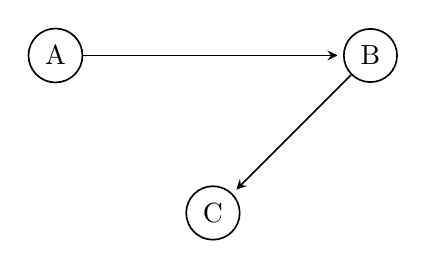
\begin{tikzpicture}[
            > = stealth, % arrow head style
            shorten > = 2pt, % don't touch arrow head to node
            auto,
            node distance = 3cm, % distance between nodes
            semithick % line style
        ]
\node[shape=circle,draw=black] (A) at (0,0) {A};
\node[shape=circle,draw=black] (B) at (4,0) {B};
\node[shape=circle,draw=black] (C) at (2,-2) {C};

 \path [->] (A) edge node[left] {} (B);
 \path [->] (B) edge node[left] {} (C);


\end{tikzpicture}
\caption{Graphs corresponding to $V = \{A,B,C\}$, $E = \{(A,B), (B,C)\}$ } \label{fig:M1}
\end{figure}

 Often times we are interested in how different nodes in a particular graph are or are not connected to one another. In this spirit we define paths.
 
\begin{definition}
A $\mathbf{path}$ $p$ between nodes $v_1, v_n \in V$ is a sequence $v_1, v_2, ..., v_n \in V$  of distinct nodes such that either $(v_i, v_{i+1}) \in E$ or $(v_i, v_{i+1}) \in E$ edge always exists between $v_i$ and $v_{i+1}$. When $v_i \rightarrow v_{i+1}$ ($(i, i-1) \in E$) for all $i \in \{1,2,...,n \}$, we say $p$ is a $\mathbf{directed \ path}$.
\end{definition}




For a directed graph $G$ and a particular node $v \in V$, we define several sets of related nodes. The \textbf{parents} of $v$, denoted $PA_v$, are the nodes with a directed edge ending at $v$, $\{j \in V | j \rightarrow v \}$ and similarly the \textbf{children}, denoted $CH_v$, of $v$ are those nodes which $v$ has a directed edge to, $\{j \in V | v \rightarrow j \}$. 

Extending these definitions, we define the \textbf{ancestors} of $v$, $AN_v$, as all the nodes from which a directed path to $v$ exists,  $\{j \in V | j \rightarrow ... \rightarrow v \}$. Likewise we define \textbf{descendants} $DE_v$ of $v$ as the nodes for which a directed path from $v$ exists,   $\{j \in V | v \rightarrow ... \rightarrow j\}$ [ref Peters chp 6.1]. With these in place, we progress to the next definition.

\begin{definition}
A directed graph $G = (V,E)$ is said to be an \emph{\textbf{directed acyclic graph}} (DAG) if for all nodes $v \in V$, $DE_v \cap AN_v = \emptyset$. That is, a directed graph is a DAG when there is never a directed path from a node to itself. 
\end{definition}

\begin{figure}
\centering
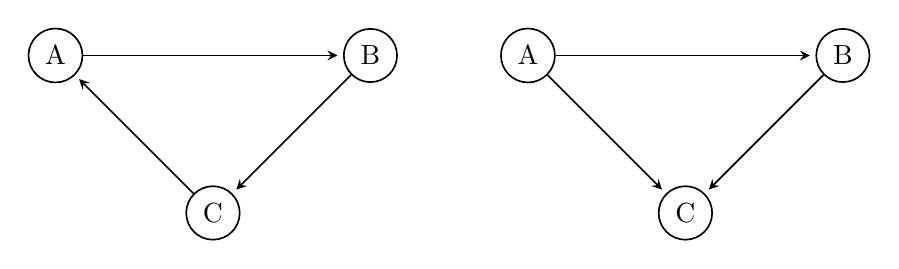
\begin{tikzpicture}[
            > = stealth, % arrow head style
            shorten > = 2pt, % don't touch arrow head to node
            auto,
            node distance = 3cm, % distance between nodes
            semithick % line style
        ]
\node[shape=circle,draw=black] (A) at (0,0) {A};
\node[shape=circle,draw=black] (B) at (4,0) {B};
\node[shape=circle,draw=black] (C) at (2,-2) {C};

 \path [->] (A) edge node[left] {} (B);
 \path [->] (B) edge node[left] {} (C);
  \path [->] (C) edge node[left] {} (A);


\node[shape=circle,draw=black] (A) at (6,0) {A};
\node[shape=circle,draw=black] (B) at (10,0) {B};
\node[shape=circle,draw=black] (C) at (8,-2) {C};

\path [->] (A) edge node[left] {} (B);
\path [->] (B) edge node[left] {} (C);
\path [->] (A) edge node[left] {} (C);
\end{tikzpicture}

\caption{Cyclic (left) and acyclic (right) graphs on the nodes $A,B,C$} \label{fig:M1}
\end{figure}

Now that we have defined DAGs, we can advance to a relevant application, Bayesian networks.

\subsection{Conditional Independence and Bayesian Networks}

The idea of conditional independence is at the basis of graphical approaches to causality. Intuitively, conditional independence statements tell us what we can \emph{ignore}. When $X \dsep Y | Z$, the conditional probability $P(x  | y, z)$ can be replaced with $P(x  | z)$, i.e. we can ignore the value of $y$ as long as we know $z$. More formally:

\begin{definition}[Conditional Independence]
Two sets of random variables $\mathbf{X}$ and $\mathbf{Y}$ are said to be \emph{\textbf{conditionally independent}} given a third set $\mathbf{Z}$ when $P(\mathbf{x}, \mathbf{y} | \mathbf{z}) = P(\mathbf{x} | \mathbf{z})P(\mathbf{y} | \mathbf{z})$. Alternatively, this condition can be formulated as $P(\mathbf{x} | \mathbf{y}, \mathbf{z}) = P(\mathbf{x}| \mathbf{z})$. We symbolize this statement as $\mathbf{X} \dsep \mathbf{Y}  | \mathbf{Z}$.
\end{definition}

 This is useful because it allows us to dramatically simplify many probabilistic expressions, making them easier to evaluate. Bayesian networks  are a popular way of encoding a particular "factorization" of a joint distribution. This requires a quick review of the chain rule for probability, an extension of the definition of conditional probability that allows joint distribution to be factored into the product of conditionals. 

\begin{definition}[Chain Rule]
A joint distribution $P(x_1, x_2, ..., x_n)$ may be factored as $P(x_1, x_2, ..., x_n) = P(x_1 | x_2, ... , x_n) P(x_2  | x_3, ... x_n) \cdots P(x_{n-1} | x_n) P(x_n)$. 
\end{definition}

Since the variables may be ordered in any way, this allows for many distinct factorizations. So, for any particular factorization, conditional independences allow it to be simplified through the removal of extraneous conditioning variables. 

\begin{example}
For a joint distribution $P(x,y,z,w)$ with the independences $X \dsep (Y,W) | Z$ and $Y \dsep W | Z$, the chain rule and conditional independence allows us to expression the joint as follows:

$$P(x,y,z,w) = P(x | y,z,w)P(y | z,w) P(z | w) P(w) = P(x | z)P(y | w)P(z | w) P(w)$$

Notice that if we had started with a different factorization, such as $P(x, y, z, w) = P(w | x, y, z) P(y | x, z) P(x | z)P(z)$ the conditional independences do not allow us to further simplify the expression. 
\end{example}

For a particular (simplified) factorization, the associated Bayesian network is the DAG formed by drawing an edge from each variable being conditioned on to the variable on the left of the conditioning bar. For our two factorizations, the associated Bayesian networks are the DAGs displayed in figure 1.4.

\begin{figure}
\centering
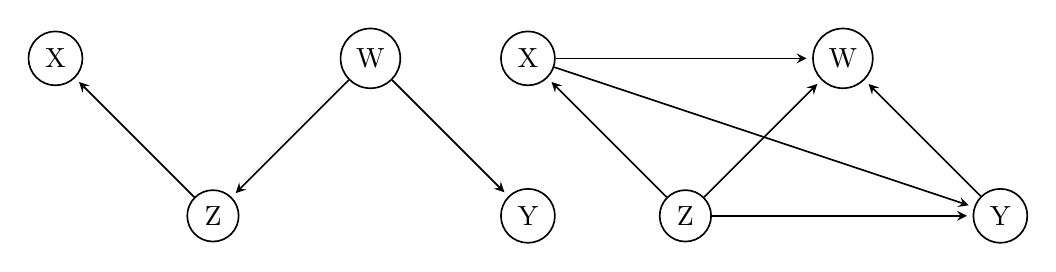
\begin{tikzpicture}[
            > = stealth, % arrow head style
            shorten > = 2pt, % don't touch arrow head to node
            auto,
            node distance = 3cm, % distance between nodes
            semithick % line style
        ]

\node[shape=circle,draw=black] (Z) at (-2,-2) {Z};
\node[shape=circle,draw=black] (X) at (-4,0) {X};
\node[shape=circle,draw=black] (Y) at (2,-2) {Y};
\node[shape=circle,draw=black] (W) at (0,0) {W};
 

 \path [->] (Z) edge node[left] {} (X);
 \path [->] (W) edge node[left] {} (Y);
 \path [->] (W) edge node[left] {} (Z);        
 
 \node[shape=circle,draw=black] (Z*) at (4,-2) {Z};
\node[shape=circle,draw=black] (X*) at (2,0) {X};
\node[shape=circle,draw=black] (Y*) at (8,-2) {Y};
\node[shape=circle,draw=black] (W*) at (6,0) {W};
 

 \path [->] (Z*) edge node[left] {} (X*);
 \path [->] (Z*) edge node[left] {} (Y*);
  \path [->] (Z*) edge node[left] {} (W*);
  \path [->] (X*) edge node[left] {} (W*);
\path [->] (Y*) edge node[left] {} (W*);
\path [->] (X*) edge node[left] {} (Y*);
\end{tikzpicture}
\caption{Bayesian networks corresponding to $P(x | z)P(y | w)P(z | w)P(w)$ (left) and $P(w | x, y, z) P(y | x, z) P(x | z)P(z)$ (right)} \label{fig:BayesNet1}
\end{figure}

This process is reversible, and given a particular Bayesian network we may "read off" the associated joint distribution as $P(x_1, ..., x_n) = \prod_{i = 1}^n P(x_i | PA_{x_i})$ \citep{Pearl_2009}. However, the real usefulness of Bayesian networks comes from way that further conditional independence relationships are encoded graphically.

\subsection{D-Separation}

Graphical structure can allow us to reason about causal and probabilistic relationships. One of the essential tools is d-separation. Graphically, d-separation statements formalize the idea that two sets of nodes can be "separated" from each other by a third set.  To develop the intuition, consider the very basic DAG $A \rightarrow B \rightarrow C$. There is exactly one directed path from $A$ to $C$, and the path passes through $B$. So to get to $C$ from $A$ you need to pass through $B$. In this way, we say that $B$ blocks the directed path from $A$ to $C$. This notion of blocking is extended to form the definition of d-separation \citep{Peters_2017}:.

\begin{definition}
Given a directed graph $G$, a path $p$ from node $v_1$ to node $v_n$ is said to be \textbf{\emph{blocked}} by a set $S$ (with $S \cap \{v_1, v_n\} = \emptyset$) if:
\begin{enumerate}
\item $v_j \in S$ and $p$ contains a $\mathbf{chain}$: $v_{j-1} \rightarrow v_j \rightarrow v_{j+1}$ or $v_{j-1} \leftarrow v_j \leftarrow v_{j+1}$, or

\item $v_j \in S$ and $p$ contains a \textbf{\emph{fork}}: $v_{j-1} \leftarrow v_j \rightarrow v_{j+1}$, or

\item $v_j \notin S$ and $DE_{v_j} \cap S = \emptyset$ and $p$ contains a \textbf{\emph{collider}}: $v_{j-1} \rightarrow v_j \leftarrow v_{j+1}$. As we will see, colliders play an especially important role in the analysis of causal DAGs.
\end{enumerate}
\end{definition}

\begin{example}
Consider a path $A \rightarrow B \rightarrow C \leftarrow D \rightarrow E$ between nodes $A$ and $E$. There are many sets that block this path. For one, there is a collider on the path. This means that any set which does not include $C$ or any elements of $DE_C$ would successfully block the path. However, we could also pick $S = \{B\}$, $S= \{D\}$, or $S = \{B,D\}$ as blocking sets since the path contains a chain at $B$ and a  fork at $D$. Importantly, if we have either of these nodes in our blocking set, we could include $C$ as well because the first blocking condition would be satisfied, even though the second would not. In fact, the only $S \subseteq \{B,C,D\}$ that would not block the path is $S = \{C\}$.
\end{example}

With blocking defined, we address d-separation. 

\begin{definition}
For a DAG $G$, two sets of nodes $A,B \in G$ are said to be  \textbf{\emph{d-separated}} by a set $S$ if all paths between $A$ and $B$ are blocked by $S$. We denote d-separation by the symbol $\perp \!\!\!\perp_G$, with the statement "In DAG $G$, $A$ is d-separated from $B$ by $S$" expressed as $A \dsep_G B | S$. 
\end{definition}

\begin{remark}
If $A \dsep_G B | S$ then $B \dsep_G A | S$
\end{remark}
\begin{example}
Consider the DAG $G$ below.

    $$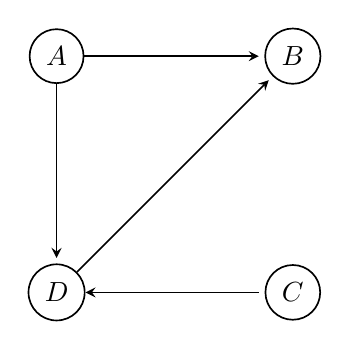
\begin{tikzpicture}[
            > = stealth, % arrow head style
            shorten > = 2pt, % don't touch arrow head to node
            auto,
            node distance = 3cm, % distance between nodes
            semithick % line style
        ]
        

        \tikzstyle{every state}=[
            draw = black,
            thick,
            fill = white,
            minimum size = 4mm
        ]

        \node[shape=circle,draw=black] (A) {$A$};
        \node[shape=circle,draw=black] (B) [right of=A] {$B$};
        \node[shape=circle,draw=black] (C) [below of=B] {$C$};
        \node[shape=circle,draw=black] (D) [left of=C] {$D$};

        \path[->] (A) edge node {} (B);
	    \path[->] (A) edge node {} (D);
	    \path[->] (D) edge node {} (B);
	    \path[<-] (D) edge node {} (C);
    \end{tikzpicture}$$
\end{example}

Which nodes can be d-separated, and by which blocking sets? Nodes which are connected by an edge cannot be d-separated. To see why, take $A$ and $B$. Although some paths between $A$ and $B$ can be blocked, the path $A \rightarrow B$ contains no nodes other than $A$ and $B$ and therefore cannot be blocked. Since there is no set that can block the path, $A$ and $B$ are not able to be d-separated. So consider $A$ and $C$, two nodes which are not connected by an edge. There are two paths between $A$ and $C$, $A \rightarrow B \leftarrow D \leftarrow C$ and $A \rightarrow D \leftarrow C$. Both of these paths include a collider. Of the four possible blocking sets, $\emptyset, \{B\}, \{D\}, \{B,D\}$, all but $\emptyset$ include a collider node for paths that are not blocked by other means. Then $A \dsep_G C | \emptyset$ and no other sets will work. What about $B$ and $C$? Again there are two paths: $B \leftarrow D \leftarrow C$ and $B \leftarrow A \rightarrow D \leftarrow C$. The second path contains a collider, and therefore is blocked by $\emptyset$, but the first path cannot be. To block $B \leftarrow D \leftarrow C$ we must have $D$ in our blocking set. So, $B \dsep_G C | D$, but we can also include $A$ since doing so will not unblock a path with a collider. Then $B \dsep_G C | D,A$.

The reason that the d-separation symbol $\dsep_G$ is so similar to the symbol for conditional independence $\dsep$ is that in any Bayesian network, the set of d-separation statement correspond to a set of conditional independences in the joint distribution. This allows us to define a notion of compatibility between particular Bayesian networks and some  joint distributions over the same variables.

\begin{definition}
For a Bayesian network $G$ over variables $X_1, ..., X_n$ and a joint distribution $P^*(x_1, ... , x_n)$ we say that $P^*$ is \emph{\textbf{compatible}} with $G$ if for every conditional d-separation statement $\mathbf{Y} \dsep_G \mathbf{Z}  | \mathbf{W}$ for $\mathbf{Y}, \mathbf{Z}, \mathbf{W} \subset \{X_1,...,X_n\}$ there is a corresponding conditional independence $\mathbf{Y} \dsep \mathbf{Z}  | \mathbf{W}$ in the distribution $P^*$.
\end{definition}

Importantly, this notion does not require that every conditional independence in $P^*$ has a corresponding d-separation in the graph. For instance, a probability distribution in which every variable in unconditionally independent from every other variable is compatible with any Bayesian network over those variables. However, the only probability distribution compatible with the Bayesian network without any edges is that fully independent distribution.  This notion of compatibility is useful for two reasons: it defines a class of distributions which are possible under a particular Bayesian network and it allows comparison between a suggested Bayesian network and available data which is alleged to conform to this network. This becomes particularly important when Bayesian networks represent a particular \emph{causal} order, as described in the next subsection.


\subsection{Structural Causal Models}
Many questions in the natural and social sciences involve understanding the way that one set of factors (e.g. genes, medicines, social policies) influence others (e.g. disease risk, mortality, childhood poverty rates). In these cases, the language and  of classical statistics is often inadequate. The tools of hypothesis testing, (linear) regression, interval estimation, etc. can tell us much about relationships in the data, but except in the highly constrained setting of randomized controlled trials, very little about cause and effect. These limitations are not just theoretical. Many longstanding controversies and debates within the sciences come down to disagreements over which factors associated with a particular outcome are causing the outcome. 

A paradigmatic example of such a controversy is over the relationship between cigarette smoking and lung cancer. Today, it is uncontroversial that smoking cigarettes (especially habitually over a long period of time) increases a person's risk of contracting lung cancer. This is a causal relationship, and we might express our belief in this relationship as a \textbf{\emph{causal model}} in which a person's risk of contracting lung cancer is a \emph{function} of a person's smoking habits (for simplicity, we  pretend that smoking is the only such causal factor).

So, let $L$ be a random variable denoting whether or not a person contracts lung cancer and $S$ be a random variable denoting smoking. Under our causal model in which smoking is the only structural cause of lung cancer, we express $L$ as a function of $S$:

$$L :=f(S, N_L),$$
$$S := N_S.$$ 

Here, the use of $:=$ denotes an assignment rather that an algebraic relationship \citep{Peters_2017} and $N_L$ is a noise term capturing random effects on lung cancer risk, and $N_S$ a noise variable for cigarette smoking. Together, these two assignments are a  structural causal model.  Now that we have an SCM, we can express the structure as a DAG. Since $L$ is assigned as a function of smoking but $S$ is not caused by any factors in our model, we would express our model as a directed edge going from $S$ to L:



$$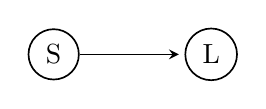
\begin{tikzpicture}[
            > = stealth, % arrow head style
            shorten > = 2pt, % don't touch arrow head to node
            auto,
            node distance = 3cm, % distance between nodes
            semithick % line style
        ]
\node[shape=circle,draw=black] (S) at (8,0) {S};
\node[shape=circle,draw=black] (L) at (10,0) {L};


 \path [->] (S) edge node[left] {} (L);
\end{tikzpicture}$$

However, historically, this causal structure was not the only one suggested to explain the association between lung cancer and smoking. One particularly illustrious detractor of this theory was British statistician R. A. Fisher, a foundational figure in modern statistics (and a heavy smoker) [ref Fisher]. In Fisher's view, there was no causal effect of smoking on lung cancer, rather, an underlying genetic factor was responsible for both a predisposition to smoking and a higher risk of developing lung cancer. So Fisher's causal model would have looked like:

$$L :=f(G, N_L),$$
$$S := f(G, N_S),$$
$$G := N_G.$$ 
Where $G$ is the genetic factor. As before, the structure of this model can be expressed as a graph:

$$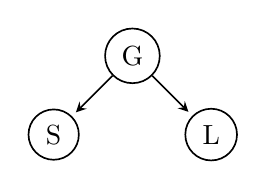
\begin{tikzpicture}[
            > = stealth, % arrow head style
            shorten > = 2pt, % don't touch arrow head to node
            auto,
            node distance = 3cm, % distance between nodes
            semithick % line style
        ]
\node[shape=circle,draw=black] (G) at (9,1) {G};
\node[shape=circle,draw=black] (S) at (8,0) {S};
\node[shape=circle,draw=black] (L) at (10,0) {L};

 \path [->] (G) edge node[left] {} (L);
 \path [->] (G) edge node[left] {} (S);
\end{tikzpicture}$$


In this way, every SCM entails a directed graph. Although it is entirely possible for an SCM to entail a graph that has cycles, we focus our attention on the case where the graph entailed is a DAG. Importantly, these two (graphical) models imply different observational joint distributions. Without having specified the functions, little can be said about the joint distribution entailed by the model, however, one important property is built in to every SCM.

\begin{definition}[Markov property]
In any SCM $C$ with entailed graph $G$, if $A \dsep_G B | S \implies A \dsep B | S$ for all disjoint sets of nodes $A,B,S$. That is, every d-separation in the graph corresponds to a conditional independence in the joint distribution. This fact is implied by the definition of SCMs and is called the \emph{\textbf{Markov Property}}.
\end{definition}

In other words, structural assignments (without cycles) induce a Bayesian network over the involved variables that the observational distribution must be compatible with. This result is a powerful tool that allows us to test how well differing causal models comport with the observational data.  Returning to Fisher's suggestion that an underlying genetic cause was responsible for the association of smoking with lung cancer, consider that by the Markov property $S \dsep L | G$. Let's assume we have a population of identical twins, some of whom were smoking discordant. Since we know that identical twins are genetically identical  we could assess whether or not smoking and lung cancer are independent within twin pairs. If not, then something must be wrong with the model. 



\section{Selection Bias and Missing Data}

Most statistical inference techniques  are designed for the case in which samples are 'representative' of the population. That is, for a finite population of size $N$, each unit in the population $X_1, ..., X_N$ are equally likely to appear in the sample. When the domain is continuous, we can extend this idea as saying that the distribution of a sampled value is the same as the "true" underlying distribution. However, this is often unattainable and therefore standard methods are inappropriate (see Chapter 4 for an overview of more appropriate methods). This problem is captured by two related phenomena: selection bias and missing data.


\subsection{Selection Bias}

Selection bias occurs whenever samples are non-representative. In the finite population case, this corresponds to some units being more likely to be sampled than others. The problem with this is serious. As a basic example, consider a sample $\tilde{\mathbf{X}}$ taken from $X_1, ..., X_N$ where each $X_i \sim \text{Bern}(p)$. If we want to estimate $p$ from a representative sample, all we need is to take the mean of our sample to get an unbiased estimator. However, if values of $X_1, ..., X_N$ are sampled such that the sampling probability of $X_i$ is larger when $X_i = 1$, then any sample, no matter how larger, will give biased estimated of $p$. 

Selection bias occurs often in practice but can be difficult to identify. Unlike the case of missing data (described in section 1.2.2), selection bias is often invisible - we don't know anything about the units that weren't sampled. The problem presented by selection bias has been a thorn in the side of empirical research for decades.

One classic example of selection bias is a 1936 presidential election poll  published in an American magazine called The Literary Digest. The election was between Franklin Delano Roosevelt, the democratic incumbent, and Alfred Landon, a republican. The Literary Digest conducted a poll drawing a sample from their readership and by telephone and using records of automobile ownership. The sample size was extremely large, with over 2 million survey respondents. Their prediction, that Landon would comfortably win the election, proved embarrassing. Not only did Landon lose, but he lost in one of the largest electoral landslides in American history:  523 electoral votes went to Roosevelt and 8 went to the Digest's predicted winner. Shortly after, the magazine ceased publication.

The precise details of what caused this failure are not fully known. One view that has become the popular explanation was that although their survey had a plenty large sample size, it was non-representative of the population as a whole. Particularly, both being subscribed to The Literary Digest and owning a telephone or car were more common among more affluent people, and so their survey skewed wealthier than the population as a whole, and therefore underestimated the proportion of voters who would vote for Roosevelt, a candidate with largely working class support. In fact, although this explanation almost certainly accounts for a part of the failure, it is unlikely to be complete. Although it is true that the survey over-sampled more affluent voters who were more likely to support Landon, a separate poll  conducted by George Gallup in 1937 found that in even voters who owned both a telephone and a car were more likely to favor Roosevelt than Landon. This means that there must have been other factors at play, and in particular, that Landon voters were more likely to return the survey than Roosevelt voters \citep{Squire1988}, \cite{lusinchi_2012}. This is called (non) response bias, and we will see that it too falls under the selection bias framework proposed here.

Selection bias can be even more subtle than this. Medical studies into the effects of a certain health conditions rely on samples of people with that condition. This can introduce a phenomenon called "survivorship bias" wherein the most severe cases are less likely to be included in the analysis because they are more likely to result in death \citep{Delgado_2008}. Of course, similar effects exist outside of medicine. 

One such case which has made its way into statistical legend concerns the work done by Abraham Wald and the Statistical Research Group (SRG) of which he was a member. The SRG was a working group of statisticians and mathematicians based at Columbia who applied statistical methods to problems faced by the American military during World War II \citep{Wallis_1980a}. Asked to reduced the number of planes being taken down by enemy fire through discovering the areas of the plane most vulnerable to damage and reinforcing them, Wald pushed back on the military's suggestion to armor the areas which (within the returning aircraft) were most affected by gunfire. In fact, Wald believed that the opposite - reinforcing the areas \emph{not} damaged in the returning aircraft - would provide the best protection. His reasoning was simple: all regions of the aircraft were similarly likely to be hit, but only those planes hit in the regions which were not essential were able to return. In other words, the full set of aircraft would have damage uniformly throughout the body of the plane, but selection into the set of returning aircraft depended on the planes not being so badly damaged that they went down \citep{Wallis_1980b}. So, the areas not damaged in the returning set must have been the areas which, if damaged, would lead to the plane going down. In this way, Wald was used additional pieces of information (uniformity of hits to the plane and the fact that downed planes had been hit in vital regions) to effectively make use of selection-biased data which otherwise would have led to dangerously wrong conclusions. 

The importance of establishing the mechanisms by which selection occurs has led to the development of graphical representations for the selection process. In the 2000s, a handful of papers were published using graphs to represent selection bias in the context of medical research \citep{Geneletti_2008} \citep{Hernan_2004} \citep{Haneuse_2009}. More recently, a group of computer scientists has generalized this work in terms of causal graphs to make substantial headway on the problem \citep{Pearl_2011} \citep{Bareinboim_2012} \citep{Bareinboim_2014}. This latter body of work is essential to our study of the problem and is reviewed in the next chapter.

\subsection{Missing Data}

Like selection bias, missing data occurs when some variables are not observed for each unit (row). Unlike selection bias, missing data can always be detected - missing values are not known, but the fact that they are missing is. In the standard missing data notation, $R_{Y_i}=1$ corresponds to the $i^{\text{th}}$ observation of a random variable $Y$ being missing. In some cases, missingness follows a very simple structure where a particular variable is not always observed (often the response variable), but covariates are available for each unit. Table 3.1 gives an example of what is meant by this. 


\begin{table}[]
\centering
\begin{tabular}{|l|l|l|l|l|l|}
Y     & $X_1$  & $X_2$  & $X_3$  & $X_4$  & $R_Y$ \\ \hline
$y_1$ & $x_{11}$ & $x_{12}$ & $x_{13}$ & $x_{14}$ & 0 \\
   -   & $x_{21}$ & $x_{22}$ & $x_{23}$ & $x_{24}$ & 1 \\
   -   & $x_{31}$ & $x_{32}$ & $x_{33}$ & $x_{34}$ & 1 \\
$y_2$ & $x_{41}$ & $x_{42}$ & $x_{43}$ & $x_{44}$ & 0
\end{tabular}
\caption{Hypothetical table representing missing data with one partially observed variable.} 
\end{table}

One example of this effect is found in studies that observe units over a long period of time, such as longitudinal studies. In these cases, researchers  have to deal with drop-out: some participants stop participating in the study before it finishes, and therefore the final outcome is not recorded for these units. Since the pre-treatment covariates are recorded for all participants before dropout occurs, only the outcome variable is missing for the units affected by dropout. This situation is a prime candidate for a technique called inverse probability weighting, which we explore in the next chapter \citep{Hernan_2004}.

Sometimes the missingness structure is more complex in that different variables are missing from different units. So while one survey respondent might answer a question on income but decline to answer a question about marital status, another might do just the opposite. A range of approaches have been developed: sometimes, rows with missing variables may be safely deleted, other times, imputation based methods are more appropriate \citep{Schafer_2002}.  For instance, survey respondents may choose not to answer some questions, but unlike in the example above, the unanswered questions can differ between units (table 3.2). In cases like this, missing data are often imputed: that is, the missing values are predicted on the basis of non-missing values, but weight based approaches like inverse probability weighting can also be applied \citep{Little_1986} ,\citep{Seaman_2011}. 

\begin{table}[]
\centering
\begin{tabular}{|l|l|l|l|l|l}
$X_1$    & $X_2$    & $X_3$    & $R_{X_1}$ & $R_{X_2}$ & $R_{X_3}$ \\ \hline
-        & -        & $x_{13}$ & 1         & 1         & 0         \\
-        & $x_{22}$ & $x_{23}$ & 1         & 0         & 0         \\
$x_{31}$ & $x_{32}$ & $x_{33}$ & 0         & 0         & 0         \\
-        & $x_{42}$ & -        & 1         & 0         & 1        
\end{tabular}
\caption{Hypothetical table representing missing data with all variables partially observed.}
\end{table}

The degree of the problem posed by missing data will depend on the form that the missingness takes. In the worst cases, a variable causes its own missingness, an effect called "self-censoring". When this happens, the problem becomes very hard for the same reason selection bias is so vexing: the sampling distribution for the missing variable will never align with the population distribution and without external data or added assumptions, there is no way to say anything about what this underlying distribution is likely to be. In more favorable cases, whether or not an entry is missing for a particular unit will only depend on the set of observed values for that unit.

Since such a wide range of missingness structures are possible, a large  literature has developed to address the problem in various contexts \citep{Schafer_2002} \citep{Heckman_1979} \citep{Little_1986}, much more so than with selection bias. Indeed, missing data has several qualities that often make it easier to handle than selection bias.  When some (but not all) features for a particular unit are not measured, those features that are measured can often inform on the features that do not. In many cases, a model can be specified to replace or "impute" the missing values \citep{Donders_2006}. In the best case, the rows with missing data can be excluded from the analysis, but unless strict assumptions are met, this method will produce biased results and potentially greatly reduce sample size. Still, even with the wealth of methods developed for handling missing data, it can be difficult or even impossible to determine which are appropriate in a particular situation \citep{Mohan_2019}. Just as with selection bias, this fact motivates the recent formulation of the missing data problem in terms of causal graphs as discussed in chapter 3.



\chapter{Graphical Representations of Selection Bias}


\section{Introduction}
In chapter 4, we give an overview of relevant methods for selection bias and missing data, including several older papers that describe sample selection graphically. However, these papers mostly made use of the graphs as conceptual models of selection for particular problems without digging into the implications of such structure in the context of particular study designs \citep{Hernan_2004}, \citep{Geneletti_2008}. Bareinboim, Tian, and Pearl's 2014 paper "Recovering from Selection Bias in Causal and Statistical Inference" provides a formulation of selection bias explicitly in terms of causal DAGs and d-separation, making it an especially important resource for developing our study of the topic. In particular, the paper provides graphical conditions (in terms of d-separations) under which a \emph{conditional} distribution $P(y | x)$ can be obtained despite selection bias. When this can be done, we say that the $P(y | x)$ can be "recovered", from a causal graph containing a selection mechanism. To illustrate the results in a practical context, we will apply the graphical approach to the Literary Digest election polling problem described in section 1.2.1.

Bareinboim et. al is broken into three sections, the first two of which are the most substantial and the focus of our attention. The first gives conditions for when a distribution can be recovered if only the biased distribution is accessible, the second gives conditions for the case where population level data is available for some variables. As we will see, the presence of external data turns out to be quite useful.

\section{Representing Selection with DAGs}

Although the topic of this paper is selection \emph{bias}, the graphical framework is really a model of selection itself. That is, it can model cases where selection does not induce bias as well as cases in which it does. Representing selection in this way requires augmenting  a structural causal model over a set of variables $\mathbf{V}$ with a node $S$ that represents inclusion in the sample. The  "manifest" (or observed) distribution is then $P(\mathbf{v} | S = 1)$, that is, the joint over our variables $\mathbf{V}$ conditioned on inclusion within the sample.  

In the finite population setting, we can think about this labeling every unit in the population with  $S=1$ if they are included in our sample and $S= 0$ otherwise. The advantage of this is that $S$ is can now be represented as another variable within the causal model, and therefore the d-separations within the associated causal graph give access conditional independences which allow selection to be ignored. This framework captures the non-biasing selection case as a selection graph in which there are no edges to $S$. In such a graph, $\mathbf{V} \dsep_G S | \emptyset$ and so $P(\mathbf{v} | S = 1) = P(\mathbf{v})$.

Finally, it should be emphasized that this method completely ignores sample size. In the real world, any sample is going to be finite and therefore any estimate of the population distribution, regardless of selection mechanism, will be subject to sampling variation. Mitigating this kind of uncertainty is not a concern of this work. Instead, it focuses purely on the effect of selection on the distribution from which the sample is being drawn. In other words, the focus is on the effect of selection on the sample as the sample becomes infinitely large.


\section{Recovering Conditionals Without External Data}
In the basic case, we only have access to a distribution corresponding to a causal graph $G$  with a set of nodes $\mathbf{V}$ equipped with a selection node $S$. The distribution $P(\mathbf{v} | S = 1)$ corresponds to the distribution of values that are selected for inclusion in the sample. 
So, returning to our election example, in the simplest model in which only income affects selection probability, our graph would look like figure 2.1. In the figure, $C$ is a random variable for the candidate a person intends to vote for, $W$ is a measure of income and $S$, as usual, is the binary variable denoting inclusion in the sample. Although in practice we would probably like to know $P(c)$, the population level distribution of intended votes, for now we restrict ourselves to $P(c | w)$, the conditional distribution of intended vote given SES. 

\begin{figure}
\begin{center}
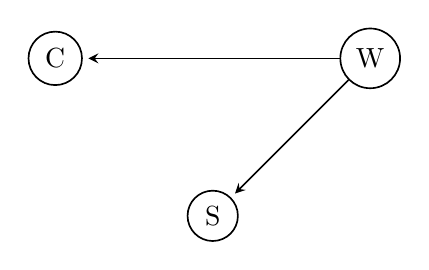
\begin{tikzpicture}[
            > = stealth, % arrow head style
            shorten > = 2pt, % don't touch arrow head to node
            auto,
            node distance = 3cm, % distance between nodes
            semithick % line style
        ]
\node[shape=circle,draw=black] (C) at (0,0) {C};
\node[shape=circle,draw=black] (W) at (4,0) {W};
\node[shape=circle,draw=black] (S) at (2,-2) {S};

 \path [->] (W) edge node[left] {} (S);
 \path [->] (W) edge node[left] {} (C);

\end{tikzpicture}
\end{center}
\caption{Graph corresponding to selection bias based on income} \label{fig:2.1}
\end{figure}

In this vein, Bareinboim et al. define \textbf{s-recoverability} as the criterion which must be satisfied for a conditional distribution such as $P(c|w)$ to be obtainable despite the selection mechanism. We reproduce their definition exactly and give an explanation of why it makes sense:

\begin{definition}
Given a causal graph $G_s$ augmented with a node $S$ encoding the selection mechanism, the distribution $Q = P(y | \mathbf{x})$ is said to be \textbf{s-recoverable} from selection biased data in $G_s$ if the assumptions embedded in the causal model render $Q$ expressible in terms of the distribution under selection bias $P(\mathbf{v} | S = 1)$. Formally, for every two probability distributions $P_1$ and $P_2$ compatible with $G_s$, $P_1(\mathbf{v} | S = 1) = P_2(\mathbf{v} | S = 1) > 0$ implies $P_1(y | \mathbf{x}) = P_2(y | \mathbf{x})$.
\end{definition}

In the example, if we are to recover $P(c | w)$  we need to express $P(c | w)$ as values derivable from $P(c, w | S = 1)$ and the conditional independences implied by the d-separations within the graph. This is what is meant by "if the assumptions embedded in the causal model render $Q$ expressible in terms of the distribution under selection bias $P(\mathbf{v} | S = 1)$", and it is worth exploring why this fairly intuitive formulation is equivalent to the formal definition given in the last sentence.

The agreement of $P_1$ and $P_2$ on the joint distribution $P(\mathbf{v} | S = 1)$ means that $P_1$ and $P_2$ produce the same observational distribution under selection bias. Therefore, when $P_1(\mathbf{v} | S = 1) = P_2(\mathbf{v} | S = 1) \implies P_1(y | \mathbf{x}) = P_2(y | \mathbf{x})$ we know that no matter the differences between $P_1$ and $P_2$, they must produce the same conditional $P(y|\mathbf{x})$. So, if this is true for every $P_1$, $P_2$, then all distributions consistent with the observational $P(\mathbf{v} | S = 1)$ produce the same $P(y | \mathbf{x})$. 

This leads to the first important result of the paper in the following theorem:

\begin{theorem}
The distribution $P(y | \mathbf{x})$ is s-recoverable from $G_s$ if and only if $S \dsep_{G_s} Y | \mathbf{X}$.
\end{theorem}

The proof of $\impliedby$ is quite long, but $\implies$ is easy. 

\begin{proof}
Assume that $S \dsep_{G_s} Y | \mathbf{X}$. Then by the Markov property, $S \dsep Y | X$ and $P(y | \mathbf{x}, S = 1) = P(y | \mathbf{x})$. So the 'recovered' distribution is simply the biased distribution.
\end{proof} 

Remarkably, this theorem means the \emph{only} time that $P(y | \mathbf{x})$ is recoverable is when $\mathbf{X}$ d-separates $S$ and $Y$ in the graph. In our application, we can see that $C \dsep_G S | W$, and so $P(c|w) = P(c|w, S = 1)$. So our study gives us direct access to the conditional distribution for candidate preference by income. This is potentially useful but restricted. What if we wish to recover a conditional distribution but do not want to condition on the full separating set? To do so, we will need external measurements.

\section{Recovery With External Data}

Sometimes a researcher will conduct a survey and collect variables on survey participants for which we know the population level distribution. For instance, the US Census collects and publishes data on occupation, race, income, and many other variables from the entire US population. If some of these variables are measured in our selection biased study, this information can be used to recover distributions that would otherwise be unavailable. 

To elaborate on this topic we will introduce a more complex model of the selection mechanism in our voter poll. As mentioned in the introduction, more recent research suggests that the assumption that income was the only variable affecting the probability of being included in the poll is not sufficient. A better explanation includes the fact that Roosevelt supporters who received the survey were much less likely to respond than Landon supporters \cite{lusinchi_2012}. This effect is called non-response bias, and is really another form of selection bias since it arises from the differing probabilities of being included in the final sample. The exact mechanism of the non-response effect in this poll is not and likely will never be known. In fact, if candidate preference directly influences the likelihood of survey response, (i.e. $C \rightarrow S$), the two nodes cannot be d-separated and we will be out of luck. Being optimistic, however, let's say we have reason to believe that another factor is the culprit. Particularly, the political party to which a survey respondent is registered could be mediating the relationship between voter preference and response probability. This model is represented in the figure below.


\begin{figure}
\begin{center}
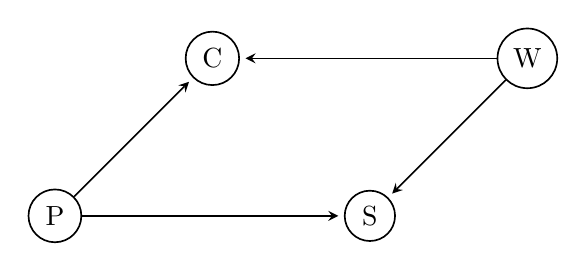
\begin{tikzpicture}[
            > = stealth, % arrow head style
            shorten > = 2pt, % don't touch arrow head to node
            auto,
            node distance = 3cm, % distance between nodes
            semithick % line style
        ]
\node[shape=circle,draw=black] (C) at (0,0) {C};
\node[shape=circle,draw=black] (W) at (4,0) {W};
\node[shape=circle,draw=black] (P) at (-2,-2) {P};
\node[shape=circle,draw=black] (S) at (2,-2) {S};


 \path [->] (P) edge node[left] {} (S);
  \path [->] (W) edge node[left] {} (S);
 \path [->] (P) edge node[left] {} (C);
 \path [->] (W) edge node[left] {} (C);
\end{tikzpicture}
\end{center}
\caption{Graph corresponding to selection bias based on income and party registration} \label{fig:2.1}
\end{figure}

Where $P$ is a binary variable denoting the party registration status of the voter. Under this model, we have a path $S \leftarrow U \rightarrow V$ which is not blocked by $W$. So $S \not \dsep_G Y | X$ and by the previous theorem, we cannot recover $P(c|w)$. Of course, we could recover $P(c | w, p)$ since $S \dsep_G V | \{W,P\}$, but assuming we are still interested in $P(c|w)$, what can be done?  

Well, we could consult the US census as well as state voter records and gather the  joint distribution for income and party registration $P(u, w)$. This is what we would call \emph{external data} since it is not affected by the selection mechanism. It turns out that in this case, we can do something. To address this situation, Bareinboim et al.  introduce a revised definition  of s-recoverability which we again reproduce and comment on. 
 
\begin{definition}
Given a causal graph $G_s$ augmented with a node $S$ encoding the selection mechanism, the distribution $Q = P(y | \mathbf{x})$ is said to be \textbf{s-recoverable} from selection bias in $G_s$ with external data over $\mathbf{T} \subseteq \mathbf{V}$ and selection biased data over $\mathbf{M} \subseteq \mathbf{V}$ if the the assumptions embedded in the causal model render $Q$ expressible in terms of the distribution under selection bias $P(\mathbf{m} | S = 1)$ and $P(\mathbf{t})$, both positive. Formally, for every two probability distributions $P_1$ and $P_2$ compatible with $G_s$, if they agree on the available distributions $P_1(\mathbf{v} | S = 1) = P_2(\mathbf{v} | S = 1) > 0$, $P_1(\mathbf{t}) = P_2(\mathbf{t})$ they must agree on the query distribution $P_1(y | \mathbf{x}) = P_2(y | \mathbf{x})$.
\end{definition}

We can see that this definition follows the same structure as the original s-recoverability definition, but is expanded to allow for the use of population level distributions. The paper's second theorem follows directly from this definition.

\begin{theorem}
If there is a set $C \subseteq V$ such that $P(\mathbf{c}, \mathbf{x})$ is measured in the population and $Y \dsep_{G_s} S | \{C,X\}$ then $P(y | \mathbf{x})$ is s-recoverable as

$$P(y | \mathbf{x}) = \sum_{\mathbf{c}} P(y | \mathbf{x}, \mathbf{c}, S = 1)P(\mathbf{c} | \mathbf{x})$$
\end{theorem}

The theorem is a straightforward application of the law of total probability.

\begin{proof}
By assumption, we have the external distribution $P(\mathbf{c}, \mathbf{x})$ and therefore $P(\mathbf{c} | \mathbf{x})$, and as usual we have $P(\mathbf{v} | S =  1)$. So can apply the law of total probability and the conditional independence $Y \dsep S | \{C,X\}$ to write:

$$P(y | \mathbf{x}) = \sum_{\mathbf{c}} P(y | \mathbf{x}, \mathbf{c}) P(\mathbf{c} | \mathbf{x}) = \sum_{\mathbf{c}} P(y | \mathbf{x}, \mathbf{c}, S = 1) P(\mathbf{c} | \mathbf{x})$$

\end{proof}

Therefore, if we wish to recover $P(c | w)$ party registration affects response probability, we can do so using the external data $P(p , w)$.

\section{A Useful Extension}
As we have seen, Bareinboim et al. is focused on the recovery of conditional distributions, i.e. $P(c|w)$. However, we would often like to have the unconditional distribution $P(v)$. Although it is only mentioned obliquely at the end of the second section, the results they prove give a simple condition for when $P(c)$ is recoverable using external data. In both sections we have seen that $P(c|w)$ was recoverable. Then, assuming that we have the external data for $P(w)$, we can use the law of total probability to write:

$$P(c) = \sum_{w} P(c|w)P(w).$$

More generally, we can formulate this result as a corollary, although it is not listed as such in the paper.

\begin{corollary}
If there exists a set $\mathbf{X} \subseteq V$ such that $P(y|\mathbf{x})$ is s-recoverable and $P(\mathbf{x})$ is available externally, then $P(y)$ is recoverable as $P(y) = \sum_{\mathbf{x}} P(y|\mathbf{x})P(\mathbf{x})$.
\end{corollary}

Being able to recover marginal distributions (rather than conditionals) will come in handy later when we compare recovery from selection bias to recovery from missing data.

\chapter{Graphical Approaches to Missing Data}

The advantages of graphical representations of selection are also found in graphical representations of missing data. As with selection, the dependence structure of missing data determines the whether a particular quantity is accessible despite missingness. This fact has long been recognized \citep{Mohan_2019}, \citep{Little_1986} and led to the widespread adoption of a classification system based on these relationships.

\section{Rubin's Taxonomy of Missing Data}

Donald Rubin's work on the missing data problem is likely the most influential out of any researcher on the topic. Rubin developed several notable techniques to address missing data including multiple imputation, the expectation-maximization algorithm, and the theory of propensity scores \citep{Little_1986}. We will discuss these methods in more details later in the next chapter, but Rubin's taxonomy \citep{Rubin_1976} of the structure of missingness is important enough to introduce now. Consider a  case with a set of variables $V_m$ potentially subject to missingness, a set $V_o$ of  fully observed variables, and a set $U$ of unmeasured variables \citep{Mohan_2013}. Define $R$ as the set containing the variables that dictates missingness among the elements of $V_m$. So if $V_m = \{Y_1, Y_2\}$ then $R = \{R_{Y_1}, R_{Y_2}\}$ where $R_{Y_i} = 1$ when $Y_i$ is missing \citep{Mohan_2013}. We consider three cases:

\begin{itemize}
\item The best case is when missingness is unrelated to all the variables, i.e. $R \dsep V_m \cup V_o \cup U$. In this case, the data are called \emph{missing completely at random} (MCAR). When this condition holds, analysis can safely be conducted on only the rows which are fully recorded.

\item If missingness depends only on the fully observed variables, i.e.  $R \dsep V_m \cup U | V_o$ we say that the data are \emph{missing at random} (MAR). Many techniques have been developed for data satisfying this condition. Overall, these techniques are more complex that those appropriate for MCAR data but are highly effective \citep{Schafer_2002}. This type of missingness is sometimes called "ignorable" not because it can actually be ignored, but because it does not pose a threat with the right techniques \citep{Pearl_2019}. Note that all MCAR data is also MAR.

\item When  the previous condition does not apply, the data are said to be \emph{missing not at random} (MNAR). This is the worst case, and is sometimes called "non-ignorable" since the techniques used to effectively adjust for MAR data cannot generally be applied. However, as we will see, the graphical approach shows that some MNAR situations are in fact recoverable.
\end{itemize}

These definitions are actually slightly adapted from Rubin's original formulation because they refer to conditional independencies among the variables rather than independencies at the unit level. That is, Rubin's original definitions allowed for data to be considered MAR when in each \emph{row}, the missingness of whichever variables were observed for the particular unit depended only on the observed values for that unit. This means that our definition is slightly more restrictive than Rubin's but this alteration makes it much more conducive to graphical representation \citep{Mohan_2013} \citep{Schafer_2002}.

To further develop the intuition, we describe variations on survey non-response satisfying each of these conditions.  Consider a very simple survey that asks each respondent for their education $E$ and their annual income $I$. Assume that age is fully observed but that income is not.

\begin{itemize}
\item (MCAR) A bug in the software used to conduct the survey means that a uniformly random selection of respondents do not receive the income question. Everyone who receives the income question answers it. 

\item (MAR) Respondents with higher levels of education are more likely to respond to the income question that those with lower education. However, within strata of education, the question is answered with equal probability.

\item (MNAR) High income respondents are less likely to respond to the income question than those with lower income. It does not matter if education is associated with non-response within the strata of income.  
\end{itemize}

However, although we can describe or display particular situations under which each condition would hold, the task becomes more difficult in practice. For one, it can be shown that it is generally not possible to test for whether or not data satisfy the missing at random condition \citep{Schafer_2002}. This limitation means that given a particular dataset containing missing values, it  (usually) is not possible to determine whether the missing values are missing at random or not without further assumptions.
\section{Graphical Innovations}

The difficulties in establishing the precise conditions under which the definitions apply as well as the conditions which allow for distributions of interest to be recovered led to the recent formulation of the missing data problem in graphical terms. As with the analogous literature we have explored on selection bias, this work also was headed by Judea Pearl and one of his graduate students, Karthika Mohan \citep{Mohan_2013} \citep{Mohan_2019}. Fortunately, familiarity with Bareinboim's framework makes understanding Mohan and Pearl's straightforward. 

As above, we consider four sets of variables: fully observed variables $V_o$, partially observed variables $V_m$, unobserved variables $U$, and the missingness variables $R$. To make the missingness process more explicit, we add to this a set of "proxy" variables $V^*_m = \{Y_i^* | Y_i \in V_m\}$ which reflect what we actually observe, such that:

$$y^*_i = \begin{cases} \text{"missing" if } r_{y_i} = 1 \\ y_i \text{ if } r_{y_i} = 0  \end{cases}$$

Notice that $Y^*_i$  is a function of $R_{Y_i}$ and $Y_i$. Since we are working with causal models, this fact implies that $PA_{Y^*_i} = \{R_{Y_i}, Y_i\}$. In this sense, $R_{Y_i}$ is not just an indicator of missingness, but the variable which enforces missingness of $Y^*$ in the causal model. With these sets constructed we define the missingness graph:

\begin{definition}
A missingness graph, denoted \textbf{m-graph}, is a causal graph $(\mathbf{V}, E)$ where $\mathbf{V} = V_o \cup V_m \cup V^* \cup U \cup R$ and $E$ is the set of edges in the graph.
\end{definition}


\begin{figure}
\centering
\begin{tikzpicture}[
            > = stealth, % arrow head style
            shorten > = 2pt, % don't touch arrow head to node
            auto,
            node distance = 3cm, % distance between nodes
            semithick % line style
        ]

\node[shape=circle,draw=black] (X) at (0,0) {X};
\node[shape=circle,draw=black, style=dashed] (Y) at (4,0) {Y};
\node[shape=circle,draw=black] (Y^*) at (2,-4) {$Y^*$};
\node[shape=circle,draw=black] (R_Y) at (2,-2) {$R_Y$};
\node[] (c) at (2,-6) {$(a)$};


 \path [->] (X) edge node[left] {} (Y);
 \path [->] (R_Y) edge node[left] {} (Y^*);
 \path [->] (Y) edge node[left] {} (Y^*);        
        
\node[shape=circle,draw=black] (X) at (6,0) {X};
\node[shape=circle,draw=black, style=dashed] (Y) at (10,0) {Y};
\node[shape=circle,draw=black] (Y^*) at (8, -4) {$Y^*$};
\node[shape=circle,draw=black] (R_Y) at (8,-2) {$R_Y$};
\node[] (c) at (8,-6) {$(b)$};

 \path [->] (X) edge node[left] {} (Y);
 \path [->] (R_Y) edge node[left] {} (Y^*);
  \path [->] (X) edge node[left] {} (R_Y);
  \path [->] (Y) edge node[left] {} (Y^*);

\node[shape=circle,draw=black] (X) at (12,0) {X};
\node[shape=circle,draw=black, style=dashed] (Y) at (16,0) {Y};
\node[shape=circle,draw=black] (Y^*) at (14,-4) {$Y^*$};
\node[shape=circle,draw=black] (R_Y) at (14,-2) {$R_Y$};
\node[] (c) at (14,-6) {$(c)$};


 \path [->] (X) edge node[left] {} (Y);
 \path [->] (R_Y) edge node[left] {} (Y^*);
  \path [->] (Y) edge node[left] {} (R_Y);
  \path [->] (Y) edge node[left] {} (Y^*);
\end{tikzpicture}

\caption{From left to right, bivariate cases of MCAR, MAR, and MNAR missing data patterns} \label{fig:Ms1}
\end{figure}

Looking at figure 3.1 (a) and (b) we have the following d-separation relationships: (a) $R_Y \dsep Y$ and (b) $R_Y \dsep Y | X$. This corresponds to the missing completely at random and the missing at random conditions, respectively. However, in the final scenario, (c), there is no set that d-separates $R_Y$ from $Y$. In each case, we have access to the joint $P(X,Y^*, R_Y)$.  By definition of $Y^*$, when we condition on $R_Y = 0$ we get $P(x,y | R_Y = 0)$, the distribution of "complete cases".

Suppose we wish to know the population level joint $P(x,y)$.  In cases (a) we have that $P(x,y | R_Y = 0) = P(x,y)$ and we are done. In case (b), the d-separation in the graph imply that $P(Y|x) = P(y| x, R_Y = 0)$ and so we apply the chain rule to get $P(x,y) = P(y|x)P(x) = P(y | x, R_Y = 0)$ and again we succeed. Indeed, our definitions of MCAR and MAR mean this method works for any such missingness structure. However, the lack of independence in the final case means that we cannot separate $Y$ from its missingness mechanism, and therefore we cannot factor out the conditional. In fact recovery is not possible in this case because $Y$ and $R_Y$ are neighbors \citep{Mohan_2013}. 

\section{Recovering Distributions Under MNAR}

With missing data, as with selection bias, what we really care about is not the distribution we have - the one subject to missingness or selection - but the population level distribution. We have seen that under the MCAR and MAR missingness conditions, the population distribution is straightforward to obtain. However, when missingness can be affected by the variables that are missing, the problem becomes much more difficult. The major task of Mohan and Pearl's papers is providing graphical characterizations for those situations in which recovery of a particular joint or condition distribution are possible or impossible. Conveniently,  definition of recovery given in Mohan et. al 2013 is equivalent to the defintion used in Bareinboim 2014,  making moving between the two easy. 

The first theorem provides a general condition under which a "query" $Q$ - meaning a probabilistic quantity such as a joint or conditional distribution - can be recovered. 

\begin{theorem}
Given a m-graph $G$ and an observed distribution $P(v^*, v_o, R)$ a query $Q$ is recoverable if $Q$ can be decomposed into an ordered factorization or a sum of such factorizations, suc h that every factor $Q_i = P(y_i | x_i)$ satisfies $Y_i \dsep (R_{X_i}, R_{Y_i}) | X_i$. Then, each $Q_i$ can be recovered as $P(y^*_i | x^*_i, R_{Y_i} = 0,R_{X_i} = 0) = P(y_i | x_i)$ \citep{Mohan_2013}. 
\end{theorem}

What this theorem is saying is fairly simple:  $Q$ can be recovered when it can be expressed as a sum or product of quantities that can be recovered individually.

\begin{example}
\begin{figure}
\centering
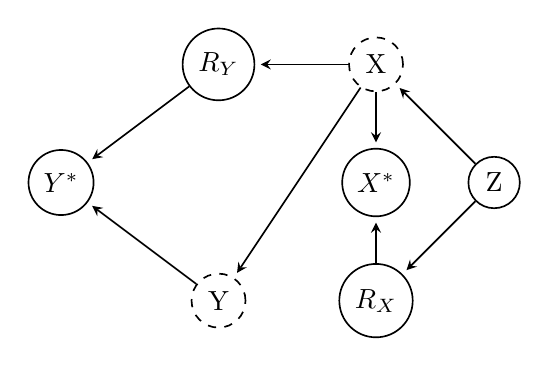
\begin{tikzpicture}[
            > = stealth, % arrow head style
            shorten > = 2pt, % don't touch arrow head to node
            auto,
            node distance = 3cm, % distance between nodes
            semithick % line style
        ]

\node[shape=circle,draw=black] (R_Y) at (0,0) {$R_Y$};
\node[shape=circle,draw=black, style=dashed] (Y) at (0,-3) {Y};
\node[shape=circle,draw=black] (Y^*) at (-2,-1.5) {$Y^*$};
\node[shape=circle,draw=black, style=dashed] (X) at (2,0) {X};
\node[shape=circle,draw=black] (X^*) at (2,-1.5) {$X^*$};
\node[shape=circle,draw=black] (R_X) at (2,-3) {$R_X$};
\node[shape=circle,draw=black] (Z) at (3.5,-1.5) {Z};

 \path [->] (X) edge node[left] {} (R_Y);
 \path [->] (X) edge node[left] {} (Y);
 \path [->] (Y) edge node[left] {} (Y^*);
 \path [->] (R_Y) edge node[left] {} (Y^*);
 \path [->] (X) edge node[left] {} (X^*);
 \path [->] (R_X) edge node[left] {} (X^*);
  \path [->] (Z) edge node[left] {} (X);
   \path [->] (Z) edge node[left] {} (R_X);
\end{tikzpicture}
\caption{A three variable MNAR m-graph} \label{fig:MNAREX}
\end{figure}

Consider the m-graph in figure 3.2. We notice that the one fully observed variable $Z$ does not d-separate $(R_X, R_Y)$ from $(X,Y)$ and therefore conclude that this m-graph corresponds to an MNAR missingness structure. However, we do have some relevant d-separations:

\begin{enumerate}
\item $X \dsep R_X | Z$
\item $Y \dsep (R_Y, R_X, Z) | X$
\end{enumerate}

Now, by the law of total probability and the chain rule for probability, we get that:

\begin{align*}
P(x,y) &= \sum_z P(x,y, z) \\
&= \sum_z P(x,y | z) P(z) \\
&= \sum_z P(y | x,z) P(x | z) P(z)
\end{align*}

When we apply our d-separations, we get that $P(y | x, z, R_Y = 0, R_X = 0) = P(y^*| x^*)$ and $P(x^*|z, R_X = 0) = P(x | z)$ and therefore:

$$\sum_z P(y | x,z) P(x | z) P(z) = \sum_z P(y^* | x^*,z, R_Y = 0, R_X = 0) P(x^* | z, R_X = 0) P(z)$$

So, we have succeed: the marginal distribution $P(x,y)$ is expressible as a sum and product of distributions which are recoverable simply using the d-separations, and so $P(x,y)$ is recoverable by theorem 4.
\end{example}

The second theorem aims a little higher: necessary \emph{and} sufficient conditions for recovering the full joint distribution $P(v_o, v_m)$.

\begin{theorem}
Given a m-graph G with no edges between $R$ nodes the joint distribution $P(v_o, v_m)$ can be recovered if and only if there is no variable $X \in V_m$ such that:
\begin{enumerate}
\item $X$ and $R_X$ are neighbors

\item $X$ and $R_X$ are connected by a path in which all intermediate nodes are colliders and elements of $V_m \cup V_o$ (i.e. at least partially observed, not an $R$ node, and not a proxy).
\end{enumerate}

When neither of these conditions apply, the joint $P(v_m, v_o)$ is recovered as:

$$\frac{P(v, R=0)}{\prod_i P(R_i = 0 | Mb(R_i), R_{Mb(R_i)} = 0)}$$

Where $Mb(R_i)$ is any \textbf{Markov blanket} for $R_i$: a set of nodes $Mb(R_i)$ such that \newline $R_i \dsep \mathbf{V} \backslash \{R_i, Mb(R_i)\} | Mb(R_i)$. In many cases, this will simply be $PA_{R_i}$. Similarly, $R_{Mb(R_i)}$ is the set of $R$ variables associated with the elements of $Mb(R_i)$ \citep{Mohan_2019}.
\end{theorem}

This final expression is a little difficult to parse, so we clarify what each component means in the following example.
\begin{example}
Lets return to the m-graph described in the previous example (figure 3.4). We check the two conditions laid out in the theorem:

\begin{enumerate}
\item The two variables subject to missingness, $Y$ and $X$ both lack an edge to their corresponding missingness node, and so the first condition is satisfied.

\item The only colliders in the graph are the two proxy nodes: $X^*$ and $Y^*$. Therefore, no path contains a collider which is an element of $V_o \cup V_m$.
\end{enumerate}

So, the population level joint $P(x,y,z)$ may be recovered as given in the theorem. This gives:

$$P(x,y,z) = \frac{P(x,y,z, R_X = 0, R_Y = 0)}{P(r_X | z)P(r_Y | x, R_x = 0)}$$
\end{example}

It is worth noting here how much stronger these results are than anything that was shown for selection bias. There, we saw that (without external data) the only distributions which can be recovered are conditionals $P(y | \mathbf{x})$ for which $Y \dsep_G S | \mathbf{X}$. When data is missing, a relatively weak condition, no self-censoring and no collider paths, is all that is needed to recover the full population distribution, as long as no edges exist between $R$ nodes. Intuitively, this gets back to the point that selection bias is much worse than missing data. With missingness, we know something about every unit, and we know what we don't know (that is, we can tell when a value is missing). Under selection bias, all we have is our biased data -  we know nothing about the units that were not sampled.

\subsection{Conditions for Non-Recoverability}

As important as it is to know when a particular quantity can be recovered, it is sometimes just as useful to know when a quantity cannot be. To this end, some attention has been paid to establishes those graphical conditions that prevent recoverability.  One of these we have already seen: theorem 5 gives that whenever $X$ and $R_X$ are neighbors or $X$ and $R_X$ are connected by a path in which all intermediate nodes are colliders and elements of $V_m \cup V_o$, the joint $P(V_m, V_o)$ is not recoverable. In fact, the necessity direction of this theorem is proven using two lemmas which are useful on their own. 

We reproduce these lemmas below:

\begin{lemma}
In the graph $X \rightarrow R_X$, $P(X)$ is not recoverable.
\end{lemma}

\begin{lemma}
If a quantity $Q$ is not m-recoverable in graph $G$, it will not be recoverable after the addition of any edge to the graph.
\end{lemma}

The second is especially useful because it says that if a quantity is not recoverable in a particular subgraph of our missingness graph, we can use lemma 2 and a simple induction to show that the quantity is not recoverable in the full graph, either. This is exactly what is done to prove that a single edge from a node $X$ to $R_X$ implies that $P(V_m, V_o)$ is not recoverable. Indeed, this makes clear that when an edge $X \rightarrow R_X$ exists, the marginal $P(\mathbf{S})$ cannot be recovered if $X \in \mathbf{S}$. 

By similar reasoning, \cite{Mohan_2014} give a similar corollary for the non-recoverability of conditionals, which we also reproduce.

\begin{corollary}
For disjoint subsets $\mathbf{X}$ and $\mathbf{Y}$,  $P(\mathbf{Y} | \mathbf{X})$ is not recoverable if one of the following conditions is true:
\item $Y$ and $R_Y$ are neighbors

\item There is a collider path connecting $R_Y$ and $Y$ such that all intermediate nodes are in $\mathbf{X}$.
\end{corollary}

This condition is obviously similar to the condition for recovering the joint, and in chapter $5$, we continue in this direction to derive more conditions for non-recovery.

\chapter{Earlier Approaches to Selection Bias and the Missing Data Problem}

In statistics and many related fields, forms of the effect we are calling "selection bias" and "missing data" have gone by many names.  In epidemiology and biostatistics, Berkson's bias (sometimes Berkson's paradox) describes a phenomenon in which two conditions that are independent at the population level become dependent within a sample as a result of both conditions affecting the likelihood of sample inclusion. This too is a kind of selection bias, as is Neyman's bias which results from survivors of a disease being selected for study but not those who died from the disease. In fact there are far more names for particular selection biases than we can describe here \citep{Delgado_2008}. One explanation for this extensive and overlapping nomenclature is that prior to the widespread use of graphical models, it was difficult to give any concise definition of selection bias that was specific enough to be useful. Selection bias is essentially about a sample with a different distribution than the population, but when that non-representivity can come from so many places this characterization is hardly useful.

Unfortunately, the different threads within the literature has caused certain terms to be overloaded. As we have seen, the tendency for types of survey recipients to respond more or less than others - (non) response bias - falls neatly into the framework of selection bias, but the same phrase is used to describe the selective answering of particular questions, which is a problem of missing data. Even the terms "missing data" and "selection bias" have this problem. For instance, James Heckman's famous "Heckman Correction"
 is widely described as a technique for dealing with selection bias. However, under our definitions, the method actually addresses missing data. 
 
In this section we will review a handful of notable earlier approaches to defining, correcting, and recognizing selection bias and missing data that have appeared within the literature, being careful to note which problem is being addressed. The purpose here is two-fold. For one, the historical background is generally useful to anyone looking for a thorough treatment of the subject. More pointedly, we will use the examples of previous methods to argue for the utility of the causal/graphical formulation used in this paper, as well as interpreting the techniques in that light.


\section{Case Analysis}

The easiest and most obvious way of "addressing" missing data is to ignore units which have missing values. There are a couple of techniques that take this approach. These techniques are widely used in practice despite significant undesirable theoretical properties \citep{Little_1986} which we discuss. In some cases, the adverse effects might be small - such as when missingness is very uncommon - but in other cases such techniques dramatically bias the results. 

\subsection{Complete-case Analysis}
In "complete-case" analysis only rows which are complete - not missing \emph{any} values - are included in the analysis. This can be thought of as deleting any row which has a missing value. There are two main problems with this approach. The first has to do with the structure of the missingness. In any case other than MCAR, the most restrictive of our taxonomy, complete case analysis produces distributions different from the population distribution \citep{Little_1986}. This is because complete case analysis is essentially a process by which data subject to missingness is made into data affected by selection bias. Since we remove any rows with missing values, we can think about complete case analysis as the process of constructing a complete data set subject to selection. Particularly, in the new data set, $S= \begin{cases}1 \text{ if } R=0 \\ 0 \text{ if } R = 1 \end{cases}$ and so in the corresponding graph, and edge would exist between each parent of an $R$ node and the selection node. Therefore, only under MCAR do we have a graph with no edges between the selection node and the rest of the graph.

The second problem with complete-case analysis is that in many contexts, it is highly inefficient \citep{Little_1986}. Consider a survey with a large number of questions and suppose we wish to know the distribution of the respondents' answers to a particular question. To conduct a complete-case analysis in such a situation would mean throwing out every row in which the respondent had failed to answer any of the many questions, even if they had answered the question of interest. In such situations, complete-case analysis results in sample sizes which are far smaller than the sample size of the original data set. This, of course, has consequences for the power of statistical tests, the size of confidence intervals, etc. 

Despite these drawbacks, complete-case analysis is very common. As above, this is mathematically appropriate when data are MCAR, but this is often not the case. Nonetheless, complete case analysis may be "good enough" for some purposes, especially when the number of excluded rows is small enough that any reasonable values for the missing data in the column of interest are unlikely to dramatically affect the analysis \citep{Schafer_2002}. 

\subsection{Available-case Analysis}

The inefficiency of complete-case analysis has an obvious (partial) remedy. Instead of deleting every row which is subject to missingness in any column, we first select the variables of interest and then only delete rows which are missing values in the corresponding columns. This method is called "available-case" analysis or sometimes "pairwise deletion" \citep{Schafer_2002}. Of course, when the number of variables of interest is close to the overall number of variables this doesn't help much, but when only a couple are needed much more data can be preserved. However, this method does nothing to address the main theoretical problem of bias: once again, data which is not MCAR is generally not appropriate for available case analysis.



\section{Imputation based Techniques} 

Imputation is the process of "guessing" missing values such that an analysis can be performed on the imputed data set. Imputation methods vary widely in their simplicity and practicality \citep{Schafer_2002}. Broadly, imputation techniques fall into one of two categories: "single" imputation and "multiple" imputation. As the names suggest, the difference between the methods is that single imputation replaces missing values with a single imputed value whereas multiple imputation replaces missing values with multiple plausible values, effectively creating multiple datasets on which the analysis can be performed. We give an overview of both approaches.

\subsection{Single Imputation}
In single imputation, the task is to replace missing values with "reasonable" guesses. There are several techniques used to generate such values all of which rely on the missingness being MCAR or MAR. We summarize them below from simplest to most complex and then discuss their advantages and disadvantages. 

\begin{itemize}
\item Mean Imputation: For a variable $Y$ subject to missingness, the missing values are replaced with the mean of the observed values of $Y$ \citep{Little_1986}.

\item Hot Deck Imputation: For a variable $Y$ subject to missingness, the missing values are replaced with the value from another row. Sometimes, this row is chosen randomly, whereas other times the row is selected based on similarity of observed covariates \citep{Little_1986}, \citep{Schafer_2002}.

\item Regression Imputation: For a variable $Y$ subject to missingness, a model $f$ is formulated based on the fully observed variables $\mathbf{X}$ is formulated and trained on the rows in which $Y$ is observed. Then, the model prediction $\hat y_i = f(\mathbf{x}_i)$ is used to imputed each missing value of $Y$ \citep{Schafer_2002}.

\item Random Regression Imputation: Same as regression imputation except rather than replacing missing $y_i$ with $\hat y_i$ we sample it from the conditional distribution implied by the model.
\end{itemize}

In general, the methods at the end of this list are preferable to the methods at the beginning. Starting with mean imputation, there are two main problems. The first is that unless the data is MCAR, the conditional (on fully observed $\mathbf{X}$) expected value  of the replacement $E[y| \mathbf{x}]$ will in general be different from the unconditional mean $E[y]$ which is used to impute. This means that when the data is not MCAR, the estimates based on the imputed data will be biased. The other problem is that because the imputed values are all the same (the mean) the variance of the imputed column will be deflated \citep{Gelman_2006}. This occurs regardless of three structure of the missingness.

Hot-deck imputation attempts to solve this problem by adding noise in the form of a random value taken from the observed values of $Y$. So, if $Y = [1,0,1,0,0, m]$ (where $m$ indicates missingness) than the missing value would be imputed as $1$ with probability $2/5$ and $0$ with probability $3/5$. This is generally preferable to mean imputation because while both methods preserve the (unconditional, observed) expected value of $Y$, but hot-deck imputation also preserves  the (unconditional, observed) variance of $Y$. However, the major problem is unaffected: as long and $Y$ and $\mathbf{X}$ are not independent, the information contained in the observed variables is wasted and estimates become biased. This means that the required assumption is very strong: for both mean imputation and hot-deck imputation are appropriate only when $Y \dsep (\mathbf{X}, R_Y)$. This means that not even MCAR missingness is enough: there cannot be any dependence between $Y$ and $\mathbf{X}$ (by the same token, MAR data could be appropriate as long as $Y \dsep \mathbf{X}$).

The solution to this problem is fairly clear: a model of the form $Y \sim X$ should be constructed to predict the missing values of $Y$ and then used to impute those values. Accordingly, this approach is called regression imputation. In the standard case, this is done using an estimate for $E[y | x]$, meaning that two rows (with $Y$ missing) which agree on $X$ will always be imputed with the same value. Analogous to the problem with mean imputation, the lack of randomness has the effect of producing exaggerating the covariance between $X$ and $Y$ \citep{Schafer_2002}. 

Fortunately, most models provide a way of adding their uncertainty back in. In the case of linear regression, the error term is assumed to be normally distributed and center at $0$ with variance that can be estimated from the residuals. In Bayesian modeling, a posterior distribution is estimated, and can be sampled from directly \citep{Gelman_2006}. Either way, missing values can be drawn according to these distributions,  fixing the covariance problems that arise in non-random regression imputation. Both of these methods require that the data is MAR rather than MCAR, meaning that with a correctly specified model, they can be justified in situations in which hot-deck and mean imputation will be inappropriate. Nonetheless, the estimation of quantities such as correlation, and especially confidence interval coverage, can still suffer even if MAR holds \citep{Schafer_2002}.
 
 
\subsection{Multiple Imputation}

The problems with single imputation methods led researchers to search for more sophisticated techniques. Donald Rubin introduced first introduced the concept of "multiple" imputation (MI) in 1977 \citep{Rubin_1977} but its classic treatment is Rubin's 1987 book on the topic.  The method has become widespread is and regarded as the best technique for imputation and among the best technique for the analysis of missing data \citep{Rubin_2019}, \citep{Schafer_2002}. Because of the large literature on the subject, attempting to fully describe the theory behind MI would go beyond the scope of this work. 

Nonetheless, we hope to give a reasonable summary of how MI works and why it is considered generally superior to single imputation. The reason that MI is referred to as "multiple" imputation is that rather than replacing each missing value with a single guess, each is replaced with a vector of length $M > 1$. In effect, this means $M$ datasets are created and analyzed separately before being combined. 

Some subtlety is involved in the way that these $M$ imputations are made. It would be possible to draw each from the posterior distribution same model (or with noise term in linear regression), however, this method would not account for the uncertainty in the terms associated with the model. To do this properly is easiest in the Bayesian  context. In that case, each parameter associated with the model has its own distribution. To construct the $M$ imputed values, we first take $M$ draws from the distribution of each parameter, creating $M$ models from which we can impute the missing values \citep{Gelman_1995}. 

The most common way of combining the $M$ datasets is simply to take the arithmetic mean of the estimates constructed in each analysis. So, in the basic setting where $Y$ is subject to missingness and $\mathbf{X}$ is fully observed such that we can model $P(R_Y = 0 | \mathbf{x}, \boldsymbol{\delta})$ with some parameters $\boldsymbol{\delta}$, the standard proceedure for constructing an estimator $\hat \theta$ with a model using multiple imputation is as follows :

\begin{enumerate}
\item Draw $\hat{\boldsymbol{\delta}}_i$ for $i \in \{1, ..., M\}$ from the distribution associated with $\boldsymbol{\delta}$.

\item For each missing value of $y$, draw $\hat y_i$ from $P(y | \mathbf{x}, \hat{\boldsymbol{\delta}}_i)$ for $i \in \{1, ..., M\}$.

\item In each of the $M$ datasets, compute $\hat \theta_i = T(y_i, \mathbf{x}_i)$ for the estimator function $T$.

\item Average the estimates as: $\hat \theta = \frac{1}{M} \sum_{i=1}^M \hat \theta_i$.
\end{enumerate} 
 
In theory, many of the desirable properties of MI rely on taking $M \rightarrow \infty$ \citep{Rubin_1996}. However, in practice, fairly small values of  $M$ (such as $20$) can work well \citep{Schafer_2002}. 
 
\section{The Heckman Correction}
James Heckman's well-cited 1979 paper "Sample Selection Bias as a Specification Error" proposes a method for overcoming "sample selection bias" that is among the most prominent selection adjustment techniques \citep{Heckman_1979}. Heckman was an economist, and his correction technique comes in the context of economic modeling, particularly linear regression models. Because it is situated within this framework, the correction is parametric - it requires the  assumption of normally distributed noise. We consider the situation in the response variable is missing for some observations. Since we are interested modeling the population values and coefficients, this poses a potential problem. The title of Heckman's paper gives a hint to his strategy: specification error refers to the omission of a relevant variable from a model. 

The method proceeds in two parts: first, a model is constructed for sample inclusion and second, an expected error term is calculated such that it can be included in the regression model to remove the bias associated with its exclusion. Understanding the specifics of Heckman's method requires substantial elaboration that is mostly irrelevant to our discussion, so in this section, we outline the approach without delving into the derivations. However, interested readers can find a detailed discussion of the technique (slightly adapted from the original to ignore finite sample concerns) in the appendix, or read Heckman's paper \citep{Heckman_1979}.

\subsection{Premise}

Although presented as a method for addressing selection bias, Heckman's technique fits better into the missing data literature. In the traditional formulation, Heckman is attempting to estimate model coefficients in the context of a finite sample. So far, we have been considering distributions rather than samples, and for the sake of continuity (as well as avoiding excessive indexing) we will present the method in the context of distributions. Fortunately, the ideas are essentially the same.

The problem is as follows: a response variable $Y$ is partially observed and assumed to fit the linear regression assumptions:

$$Y = \mathbf{X} \boldsymbol{\beta} + \epsilon$$

Where as usual $\epsilon \sim N(0, \sigma^2)$.

 for an observed vector of variables $X$. The missingness of $Y$ is governed by a variable $Z$ which is not observed but also assumed to follow the linear regression assumptions for another  set of fully observed covariates $\mathbf{W}$ (often assumed to be a superset of $\mathbf{X}$) such that:
 
$$Y = \mathbf{W} \boldsymbol{\delta} + \tau$$

With $(\epsilon, \tau) \sim N(\mathbf{0}, \boldsymbol{\Sigma})$ for some covariance matrix $\boldsymbol{\Sigma}$.  Particularly, missingness occurs when $Z$ exceeds some particular value $c$, i.e. $R_Y = 1$ when $Z > c$. Without losing generality, it is often assumed that $c = 0$. 

Heckman's insight was that under this set-up, the biased estimate of $\beta_0$ produced by running a regression on only the fully observed rows can be treated as a "specification error" - the failure to include a relevant variable. This value can be computed analytically as $\frac{\phi(\frac{-\mathbf{W} \boldsymbol{\delta}}{\sigma_\tau})}{1 - \Phi(\frac{-\mathbf{W} \boldsymbol{\delta}}{\sigma_\tau})}$ where $\sigma_\tau$ is the standard deviation of $\tau$, $\phi$ is the standard normal pdf and $\Phi$ is the standard normal cdf. The details of this calculation are somewhat involved and therefore are located in the appendix alongside some examples. 

However, with this out of the way, the method is simple to implement. There are three steps:

\begin{enumerate}
\item  First, a probit model is employed to estimate $\frac{\boldsymbol{\delta}}{\sigma_\tau}$, i.e. $P(S = 1 | \mathbf{W}) = \Phi(\frac{ \mathbf{W} \boldsymbol{\delta}}{\sigma_{\tau}})$. 

\item This estimated quantity is used to get an estimate of  $\frac{\phi(\frac{-\mathbf{W} \boldsymbol{\delta}}{\sigma_\tau})}{1 - \Phi(\frac{-\mathbf{W} \boldsymbol{\delta}}{\sigma_\tau})}$.

\item The estimate of $\frac{\phi(\frac{-\mathbf{W} \boldsymbol{\delta}}{\sigma_\tau})}{1 - \Phi(\frac{-\mathbf{W} \boldsymbol{\delta}}{\sigma_\tau})}$ is included in the corrected model $Y = \mathbf{X} \boldsymbol{\beta} + \frac{\phi(\frac{-\mathbf{W} \boldsymbol{\delta}}{\sigma_\tau})}{1 - \Phi(\frac{-\mathbf{W} \boldsymbol{\delta}}{\sigma_\tau})} + \epsilon$. The coefficient on $\frac{\phi(\frac{-\mathbf{W} \boldsymbol{\delta}}{\sigma_\tau})}{1 - \Phi(\frac{-\mathbf{W} \boldsymbol{\delta}}{\sigma_\tau})}$ is then an estimate of $\gamma \sigma_\tau = \rho \sqrt{\sigma_\epsilon}$. In this model, the estimate of the intercept,$\hat \beta_0$, is now consistent, meaning that as the sample size increases $\hat \beta_0 \rightarrow \beta_0$ in probability.
\end{enumerate}


\subsection{Graphing Heckman}
Although Heckman's method makes assumptions which are not captured by a causal graph (such as normality of $\epsilon$, $\tau$), it is still instructive to supply the graph that Heckman's setup induces. One thing to note: when $Y$ is not observed, its residual cannot be calculated. Therefore, we include $R_\epsilon$ as a node in the graph as a child of $Z$ with the idea that $\epsilon$ is not observed when $Z  > c$.

\begin{figure}[H]
\begin{center}
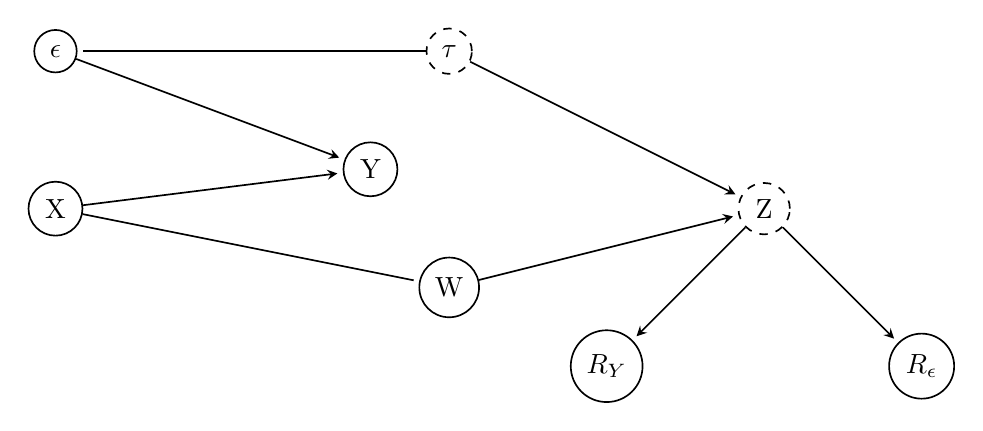
\begin{tikzpicture}[
            > = stealth, % arrow head style
            shorten > = 2pt, % don't touch arrow head to node
            auto,
            node distance = 3cm, % distance between nodes
            semithick % line style
        ]
\node[shape=circle,draw=black] (X) at (0,0) {X};
\node[shape=circle,draw=black] (Y) at (4,.5) {Y};
\node[shape=circle,draw=black, style=dashed] (Z) at (9,0) {Z};
\node[shape=circle,draw=black] (S) at (7,-2) {$R_Y$};
\node[shape=circle,draw=black] (W) at (5,-1) {W};
\node[shape=circle,draw=black] (E) at (0,2) {$\epsilon$};
\node[shape=circle,draw=black] (R_E) at (11,-2) {$R_\epsilon$};
\node[shape=circle,draw=black, style=dashed] (T) at (5,2) {$\tau$};

 \path [->] (X) edge node[left] {} (Y);
 \path [->] (E) edge node[left] {} (Y);
  \path [->] (T) edge node[left] {} (Z);
    \path [->] (W) edge node[left] {} (Z);
        \path [->] (Z) edge node[left] {} (S);
                \path [->] (Z) edge node[left] {} (R_E);
   \path [-] (T) edge node[left] {} (E);
   \path [-] (X) edge node[left] {} (W);
\end{tikzpicture}
\end{center}
\caption{PDAG corresponding to the structural equations in Heckman's set up. We leave arrows off the edges between $\epsilon$ and $\tau$ and between $X$ and $W$ since the directions are not given by the structural equations. Dashed circles indicate unobserved variables.}
\end{figure}

Several insights can be gained from viewing this graph in the light of more recent methods. First, since $Y \dsep_G R_Y | Z$, if $Z$ were observed it would be possible to recover $P(y | x)$ (and therefore $E[y | x]$) from $P(x,y) = \sum_z P(x,y | z)P(z) = \sum_z P(x,y | z, R_Y = 0)P(z)$. However, when $Z$ is not observed, the chain of unobserved variables $\epsilon, \tau, Z$ between $Y$ and $R_Y$ mean that $P(y | x)$ is not recoverable.

One fact that comes up during the derivation is and is also clear in the graph is that when the edge between $\epsilon$ and $\tau$ is inactive, the sampling procedure will not affect the estimates since  $Y \dsep_G S | X$ and so $P(y| x) = P(y|x, R_Y = 1)$. Since $(\epsilon, \tau)$ is bivariate normal, this occurs exactly when $\epsilon$ and $\tau$ are uncorrelated. 


\section{Weight Based Approaches}

Another family of techniques worth mentioning is the broad array of weight based estimators. Versions of the technique are old and have uses well outside of adjusting for selection bias a \citep{Horvitz_1952}, but we give an interpretation particularly suited to our definition of selection bias. Given a particular (non-representative) sample, the goal is to construct a 'new' sample which follows the population distribution by giving the rows different 'weights' depending on their probability of being included in the sample. 

Probability weighting techniques are associated with adjusting for confounding bias for causal inference, but methods have been developed that address selection bias as well \citep{Correa_2017}. They are  widely applied in survey statistics, where the goal is to generalize the results of the survey to some broad group such as likely voters, American adults, or members a a particular religious group. If costs and logistical concerns are ignored, the survey would be conducted using a "simple random sample" of the target population - that is - a sample in which every member of the target population is equally likely to be included in the sample. Unfortunately, this is only rarely possible. Often times, some members of the population are much hard to reach than others, which was (part of) the problem we saw earlier with the Literary Digest survey before the 1936 election. When this happens, some units in the population are more likely to be sampled than others, and it is helpful to notate this by assigning the $i^{th}$ member of the population of size $N$ has sampling probability $p_i$ \citep{Valliant_2018}.

For instance, in a simple random sample of size $n$, we have that $p_i = \frac{n}{N}$ for all $i \in \{1,...,N\}$. Notice that $\sum_i p_i  = n$ rather than $1$. Then, regardless of the sampling pattern, each unit is assigned a weight $w_i = \frac{1}{p_i}$ called, appropriately, the inverse probability of selection weight.

However, the question remains about how such weights might be calculated. Sometimes, the specifics of the survey design allow for weights to be calculated, and in others, models (such as logistic regression) are specified \citep{Valliant_2018}. In either case, formulating selection graphically makes clear exactly what quantity needs to be estimated to construct the weights. In general, $p_i$ could depend on almost any factor associated with the unit: income, age, name, location, primary language, etc. could all conceivably impact the likelihood  of a person being included in the sample. When a graphical model is specified, we simplify the problem to estimating $p_i = P(S = 1 | PA_S)$. 

External data is often used to help calculate this value. One such approach is outlined by Pew Research, one of the most well known American polling organizations. Pew uses a combination of census data and representative survey data to construct a "synthetic population" distribution over a carefully selection set of measures that mirrors the real demographic profile of the United States. Then, the sampled units are compared with the synthetic population and a random forest model is fit to estimate the probability of sample inclusion for each of the units. Regardless of how weights these calculated, many quantities can be estimated without bias as long as the weights are calculated correctly (often a challenge). If a variable $Y$ is measured in each of the $n$ units, we can estimate $E[Y]$ using the weights as:

$$\hat y = \frac{\sum_j^n }{\sum_j^n w_j}$$

Much more complex estimators can also be constructed such as for linear regression or generalized linear models \citep{Haneuse_2009}. Additionally, similar techniques can be applied for missing data. There, the weights are derived from probability of missingness, which can best estimated directly from the data (under the MAR assumption)  \citep{Seaman_2011}.

\subsection{Probability Weighting for Distributions}

For most of this paper, our primary concern is recovering entire distributions affected by selection bias rather than making a particular estimator consistent. Less work exists on this question, but, a similar technique which also relies on $P(S=1 | \mathbf{v})$ can be applied. 

When dealing with distributions affected by selection bias, our target distribution is $P(\mathbf{v})$ and we have access to $P(\mathbf{v} | S = 1)$. Then, Bayes rule gives that \citep{Cortes_2008}:

$$P(\mathbf{v}) = \frac{P(\mathbf{v}  | S = 1)P(S = 1)}{P(S=1 | \mathbf{v})} = P(\mathbf{v}  | S = 1) \frac{P(S = 1)}{P(S=1 | PA_{S})}$$

So, with knowledge of $P(S=1 | PA_S)$ and $P(S = 1)$ we can fully recover $P(\mathbf{v})$ by again multiplying by the target distribution. 

So clearly knowing $P(S = 1)$ and $P(S = 1|x)$ is quite powerful. As with Heckman, this method requires information about the selection mechanism, but doesn't assume population level information about the other variables. This is a real difference between inverse probability weighting or the Heckman correction and the graphical approaches we examine next. However, unlike Heckman, inverse probability weighting does not require  assumptions about the parametric structure of the data and instead works with non-parametric values.   

\section{Getting Graphical}


By the first decade of the 2000's, Pearl's causality framework had become well-known not just in computer science but in applied fields as well. Accordingly, this period marks the first attempts to formulate selection bias in graphical terms. Specifically, we discuss two influential papers that drawn on Pearl's work.

\subsection{Hern\'an et. al}

Miguel Hern\'an's 2004 paper "A Structural Approach to Selection Bias" sets out to distinguish between selection bias and other problematic features of studies using the logic of causality. Although some other work had used DAGs to represent selection into a study \citep{Robbins_2001}, \citep{Pearl_1995}, Hern\'an's paper went further in that it gave an explicitly graphical interpretation of presence bias caused by selection. Hern\'an, an epidemiologist, is particularly concerned with presence of selection bias within case-control and cohort studies, and his paper proceeds primarily by drawing on examples of such studies in which selection bias is a problem. As is often the case in medical studies, the random variables considered are mostly binary, meaning that instead of looking for conditional distributions in general, related quantities such as risk ratios or odds ratios are considered. However, the concepts are very similar.

The core of Hern\'an's argument is that selection bias occurs when we \emph{condition on common effects} of the exposure (treatment) and the outcome through selection. That is, the effect of the treatment $X$ on the outcome $Y$ is affected by selection bias when both selection and the treatment depend on $X$ or an ancestor (cause) of $X$.  In Barenboim's  2014 paper, we saw a version of this statement in theorem 1: $P(y|\mathbf{x})$ is recoverable as $P(y|\mathbf{x}, S = 1)$ when $Y \dsep_G S | X$. By the definition of d-separation,  This definition can be contrasted with confounding, which has its roots in common \emph{causes}. Hern\'an gives an simple example illustrating what is meant by this which we reproduce. 

\begin{figure}[H]
\begin{center}
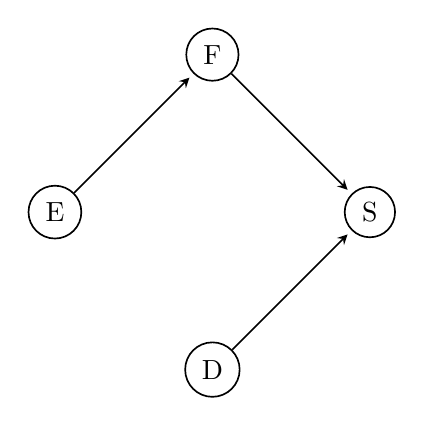
\begin{tikzpicture}[
            > = stealth, % arrow head style
            shorten > = 2pt, % don't touch arrow head to node
            auto,
            node distance = 3cm, % distance between nodes
            semithick % line style
        ]
\node[shape=circle,draw=black] (E) at (0,0) {E};
\node[shape=circle,draw=black] (F) at (2,2) {F};
\node[shape=circle,draw=black] (D) at (2,-2) {D};
\node[shape=circle,draw=black] (S) at (4,0) {S};


 \path [->] (E) edge node[left] {} (F);
 \path [->] (D) edge node[left] {} (S);
  \path [->] (F) edge node[left] {} (S);
\end{tikzpicture}
\end{center}
\caption{Study design for the Hern\'n's example}
\end{figure}

Here, $E$ is the treatment, estrogen supplements, $F$ denotes women who fractured their hips, and $D$ represents having a heart attack. We want to know if estrogen use increases the risk of having a heart attack. The study participants were gathered in such that the controls, the women who did not have a heart attack, were disproportionately women who had fractured their hips. This could be because the sample was taken from a particular hospital. Since estrogen use decreases a woman's risk of breaking her hip, this means that women taking estrogen are underrepresented within the controls. So, if we look at $P(d | e, S = 1)$ then we will find a positive relationship between $F$ and $E$ since selection into the study is a caused by both estrogen use (indirectly through decreased hip factors) and having a heart attack. So by selecting our sample in the way that we have, we have conditioned on a common effect of both the treatment and the outcome, biasing our inferences. In the reader's digest survey, 

Although Hern\'an's work was important in categorizing selection bias through graph structure, the paper was not primarily concerned with correcting for selection bias. There is a short section on how to overcome such bias, but it was limited to inverse probability weighting, a technique we have already discussed. Fortunately, the next paper we examine does. 



\subsection{Geneletti et. al}

Following up on Hern\'an's work characterizing selection bias, another  group of epidemiologists,  Geneletti et. al give a method for correcting selection bias in retrospective case-control studies using DAGs and conditional independence \citep{Geneletti_2008}. In spirit this is very similar to Bareinboim's work but limited to a specific study design such that further assumptions can be leveraged.  We now briefly review the structure of a retrospective case-control study. 

Unlike experiments where treatments are assigned randomly and outcomes measured after treatment, or cohort studies where individuals are tracked over a long period to see if they develop a disease, retrospective case-control studies (often just called case-control studies) select individuals for sample inclusion \emph{after} they have contracted a disease \citep{Woodward_1999}. Two groups are selected: one which has a particular disease/condition and one which does not. Then, covariates are gathered for both groups, with the hope of discovering some factors which are more common in one group that the other. So for instance, we could gather a sample of lung cancer patients and another of adults without lung cancer. We would likely discover that after adjusting for relevant demographic factors (age, sex, SES, etc.) smoking was more common in the lung cancer group and then construct an estimate of the risk ratio for smoking and lung cancer. However, this kind of study is particularly susceptible to selection bias \citep{Woodward_1999} \citep{Geneletti_2008}. This can happen for different reasons, but one of most prominent is that the treatment (smoking, in our example) might cause patients to be admitted to the hospital for a reason unrelated to lung cancer, but upon their admission be discovered to have lung cancer. In this way, we might see a dependence between lung cancer and smoking that is caused by smoker's greater likelihood to be diagnosed.  Similarly, when both cases and controls are selected from the hospital Berkson's bias could create a false negative association \citep{Hernan_2004}.  

Much like the first theorem of \cite{Bareinboim_2014}, Geneletti goes about recovering a conditional distribution by constructing a "bias breaking" set that d-separates (though they do not use the term) the selection node from treatment. The paper uses a similar Hern\'an's, concerning the effect of estrogen use on an unspecified outcome $Y$ where vaginal bleeding $B$ is a symptom of estrogen use and a cause of selection.


\begin{figure}[H]
\begin{center}
\begin{tikzpicture}[
            > = stealth, % arrow head style
            shorten > = 2pt, % don't touch arrow head to node
            auto,
            node distance = 3cm, % distance between nodes
            semithick % line style
        ]
\node[shape=circle,draw=black] (E) at (0,0) {E};
\node[shape=circle,draw=black] (Y) at (2,2) {Y};
\node[shape=circle,draw=black] (B) at (2,-2) {B};
\node[shape=circle,draw=black] (S) at (4,0) {S};


 \path [->] (E) edge node[left] {} (F);
 \path [->] (Y) edge node[left] {} (S);
   \path [->] (E) edge node[left] {} (D);
  \path [->] (B) edge node[left] {} (S);
    \path [-, dashed] (B) edge node[left] {} (Y);
\end{tikzpicture}
\end{center}
\caption{Study design for the Geneletti's example. The undirected dashed line indicates that the edge may or may not be present and could be oriented in either direction.}
\end{figure}

As is common in medical studies, the goal is to estimate the "odds ratio", $\frac{P(E = 1 | Y =1)P(E = 0 | Y = 0)}{P(E = 1 | Y = 0)P(E = 0 | Y = 1)}$, which can be derived directly from the conditional $P(e | y)$.  The authors write that when $E$ and $S$ are associated (i.e. $E \not{\dsep_G} Y$) bias can be introduced to the this odds ratio estimated using $p(y | e, S = 1)$. However, as we can see from the graph, $E \dsep_G S | (Y,B)$, or in the authors' words, $(Y,B)$ is a "bias breaking set". They further assume that $P(b | y)$ is known as additional data, and therefore, 

$$P(e | y) = \sum_b P(e | y, b)P(b | y) =  \sum_b P(e | y, b, S = 1)P(b | y)$$

Although they do not attempt to generalize their result to more general graphical structures, it is worth noting that this result is closely related to the external data recovery theorem in \citep{Bareinboim_2014}. 
\chapter{Simultaneous Selection Bias and Missing Data}
In Chapters 2 and 3 we discussed the contributions of two groups of researchers on the related topics of graphical characterizations of selection bias and  graphical characterizations of missing data. Although these literatures share terminology, approach, and even authors, there has been no effort to date to apply the machinery of graphical models to cases in which both selection bias and missing data are present. We feel that this is a gap in the research that should be filled. 


As we have argued in the previous chapters, missing data and selection bias are fundamentally related. In both cases we have some available data which doesn't quite match with what the true population data would look like. Indeed, many of the situations in which selection bias is a major concern are also canonical cases for missing data. For instance, almost any survey must contend with selection bias: both the people who are approached for the survey and the people who when approached actually respond are likely to differ from those who are not. In many observational medical studies, the study group is taken from a hospital. This can present a couple problems: Berkson's bias means that such a sampling procedure can create spurious negative correlations between conditions, and in the United States, hospitalized people are likely to be higher income than those with similar conditions who are not in the hospital. Often, these studies observe units over a long period of time, leading to one of the other classic forms of missing data: study drop-out (censoring). Clearly, it would be desirable to have a framework which describes these related situations in unified terms.

Fortunately, the existing graphical approaches to selection bias  and missing data  are highly compatible with each other. 

\section{Basics}

In fact, we can define a selection-missingness graph (sm-graph) exactly as we would want. Just as in the selection or missingness graphs, we define recoverability, sticking close to the definitions in \cite{Mohan_2013} and \citep{Bareinboim_2014}.

\begin{definition}[sm-recoverability]
A relation $Q$ (such as a conditional or marginal probability) is recoverable in $G$ if and only if $Q$ can be expressed in terms of the observed distribution $P(V^*_m, V_o, \mathbb{R}| S=1)$. Formally, for every two probability distributions $P_1$ and $P_2$ compatible with $G$, $P_1(V^*_m, V_o, \mathbf{R}| S=1) = P_2(V^*_m, V_o, \mathbf{R}| S=1)$ implies that $P_1(Q) = P_2(Q)$.
\end{definition}
\section{Easy Facts}


This set-up lends itself to a handful of obvious but nonetheless potentially useful facts about recovery from an sm-graph. First of all, as we discussed in the section on complete-case analysis, "deleting" every row which has missing values can be thought of as imposing an additional selection condition on the data generating process. This gives us a simple sufficient (but far from necessary) condition for recovering a distribution. The graphical interpretation of this fact is encoded in the following definition.


\begin{theorem}
In an sm-graph $G$ with no edges between the $R$ variables and $S$,  no edges between a variable and its associated missingness node, and no collider paths, the necessary and sufficient condition for recovering $P(y | \mathbf{x})$ is that $Y \dsep_G S | \mathbf{X}$.
\end{theorem}

\emph{Proof} $\implies$ We first follow the proof of theorem $3$ from \cite{Mohan_2019} to show that $P(v | S = 1)$ is recoverable. We have that:

\begin{align*}
P(\mathbf{v},  \mathbf{R} = 0 | S = 1) &= P(\mathbf{v} | S = 1) P(\mathbf{R} = 0 | \mathbf{v}, S = 1) \\
&= P(\mathbf{v} | S = 1) P(\mathbf{R} = 0 | \mathbf{v})
&= P(\mathbf{v} | S = 1) \prod_i P(R_i = 0 | pa_{R_i})
\end{align*}

Giving $P(\mathbf{v} | S = 1) = \frac{P(\mathbf{v},  \mathbf{R} = 0 | S = 1)}{\prod_i P(R_i = 0 | pa_{R_i})} = \frac{P(\mathbf{v},  \mathbf{R} = 0 | S = 1)}{\prod_i P(R_i = 0 | pa_{R_i}, R_{PA_{R_i}})} $, much as in the original. The only difference comes in the second equality.  This is immediate from $\mathbf{R}  \dsep S | \mathbf{v}$, which is true by the assumption that there are no edges between $S$ and and $R$ node. So, since $P(\mathbf{v} | S= 1)$ is recoverable, we can ignore the missingness and directly apply the result from \citep{Bareinboim_2014}.






A more useful idea comes from considering that we can essentially treat the missingness and selection mechanisms as separate. That is, if we can recover the joint from missing data when selection is not present, i.e. $P(v_m, v_o )$, then we can recover $P(v_m, v_o | S = 1)$ in the sm-graph. This means that in such cases we then look to the conditions for recovery in the selection graph while ignoring the missingness mechanisms.

\begin{theorem}
In an sm-graph $G$ with no edges between the $R$ variables and $S$ and such that $PA_S \subset V_o$, a quantity $Q$ derivable from $P(v_o, v_m)$ is recoverable if and only if $Q$ is s-recoverable in $G \backslash (\mathbf{R}  \cup V_m^*)$ and $Q$ is m-recoverable in $G \backslash S$.
\end{theorem}

\emph{Proof} (If) Assume that $Q$  is s-recoverable in $G \backslash (\mathbf{R}  \cup V_m^*)$ and $Q$ is m-recoverable in $G \backslash S$. First we decompose 

\begin{align*}
P(v_m^*, v_o, \mathbf{r} | S = 1) &= P(v_m^*, v_o, |  \mathbf{r}, S = 1) P( \mathbf{r} | S= 1) \\
&= \frac{P( \mathbf{r}, S = 1 | v_m^*, v_o)P(v_m^*, v_m^*) P( \mathbf{r} | S= 1)}{ P(\mathbf{r} , S= 1)} \\
&= \frac{P(S = 1 | v_m^*, v_o)P( \mathbf{r} | v_m^*, v_o)P(v_m^*, v_m^*) P( \mathbf{r} | S= 1)}{P( \mathbf{r} , S= 1)} \\
&= \frac{P(S = 1 |  v_o)P( \mathbf{r}, v_m^*, v_o) P( \mathbf{r} | S= 1)}{P( \mathbf{r} , S= 1)} \\
&= \frac{P(v_o | S = 1) P(S = 1) P( \mathbf{r}, v_m^*, v_o) P( \mathbf{r} | S= 1)}{P(v_o) P(\mathbf{r} | S= 1)P(S = 1)} \\
&= \frac{P(v_o | S = 1) P( \mathbf{r}, v_m^*, v_o) }{P(v_o)}  
\end{align*}

Consider two probability distributions $P_1, P_2$ with $P_1(v_m^*, v_o, \mathbf{r} | S = 1) = P_2(v_m^*, v_o, \mathbf{r} | S = 1)$. By the above, 

(Only if) Without loss of generality, assume that $Q$ is not s-recoverable in $G \backslash (\mathbf{R} \cup V_m^*)$. Then there exist two probability distributions $P_1$ and $P_2$ such that $P_1(v_m, v_o | S = 1) = P_2(v_m, v_o | S = 1)$ but $P_1(Q) \neq P_2(Q)$. Then, define $P'_1, P'_2$ as $P'_1(v_m, v_o, \mathbf{r} | S = 1) = P_1(v_m, v_o | S = 1)P(\mathbf{r})$ and $P'_2(v_m, v_o, \mathbf{r} | S = 1)P_2(\mathbf{r})$ are compatible with $G$ (when all edges to and from $\mathbf{R} \cup V_m^*$ are inactive), we have $P_1()$

\begin{theorem}
A distribution $P(X)$ is not m-recoverable if there exists $Y \in PA_{R_X}$ such that $Y$ is self-censoring ($Y \in PA_{R_Y}$) and $Y$ is a neighbor of $X$.
\end{theorem}

\emph{Proof} (Similar to  \cite{Mohan_2013} section 5.5)The proof requires a lemma proven in \cite{Mohan_2013}, copied below.


With this result in mind, consider figure 5.1.

\begin{figure}
\centering
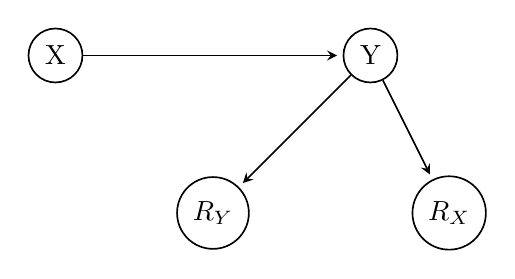
\begin{tikzpicture}[
            > = stealth, % arrow head style
            shorten > = 2pt, % don't touch arrow head to node
            auto,
            node distance = 3cm, % distance between nodes
            semithick % line style
        ]

\node[shape=circle,draw=black] (X) at (0,0) {X};
\node[shape=circle,draw=black] (Y) at (4,0) {Y};
\node[shape=circle,draw=black] (R_X) at (5,-2) {$R_X$};
\node[shape=circle,draw=black] (R_Y) at (2,-2) {$R_Y$};
 

 \path [->] (X) edge node[left] {} (Y);
 \path [->] (Y) edge node[left] {} (R_Y);        
  \path [->] (Y) edge node[left] {} (R_X);      
\end{tikzpicture}
\caption{Case in which $P(X)$ is not recoverable} \label{fig:NonRec}
\end{figure}

The lemma gives that if $P(X)$ is not recoverable in the graph ($G$) displayed in figure 5.1, $P(X)$ is non-recoverable in \emph{any} missingness graph which contains $G$ as a subgraph. Then, it is sufficient to provide a direct counter-example. We construct two probability distributions, $P_1, P_2$ compatible with $G$ such that $P_1, P_2$ agree on the observed distributions but $P_1(x) \neq P_2(x)$. Since there is only one d-separation in $G$ ($X \dsep (R_X, R_Y) | Y$) the only condition that must hold for compatibility is that $P_i(x, y, r_x, r_y) = P(x | y)P(y, r_x, r_y)$.  

Claim: A marginal distribution $P(\mathbf{X})$ can be recovered in m-graph $G$ if and only if $P(\mathbf{X})$ can be recovered in the m-graph $G'$ formed by deleting any self-censoring node $Y$ and its associated $R_Y$ and redrawing replacing every edge from $Y$ to a missingness node with an edge from each parent and child of $Y$ in $V_m \cup V_o$ to that missingness node.

$\implies$ We prove the condition in three cases.

Case 1: $Y$ has no parents and no children in $V_m \cup V_o$. In this case, $Y \dsep_G (V_m \cup V_o \backslash Y) | \emptyset$

\section{External Data Recovery}

In overcoming selection bias,  access to population distributions for a subset of the variables has been shown to be useful. In the graphical methods outlined in chapter 2, separate graphical conditions were developed for recovery. Older methods for selection bias adjustment such as survey weighting also depend on knowing population distributions. However, none of the recent graphical work on missing data has addressed the utility of external data in that context. Intuitively, we can imagine it might: if data for one variable is missing, it makes sense that knowing what that data \emph{would} look like if it were not subject to missingness. In fact, this is true. Consider the following example:

\begin{example}
In figure 5.1, we display what is sometimes called a "hard" case of MNAR missingness: $Y$ contributes to its own missingness (self-censoring). Without external data, we could neither recover $P(x,y)$ or $P(y|x)$. We could recover $P(x | y)$ as $P(x | y) = P(x | y^*, R_Y = 0)$. However, if we assume that we know $P(y)$ then we simply apply Bayes' rule to get:

$$P(y | x) = \frac{P(x|y)P(y)}{P(x)}$$

We can also recover the joint $P(x,y)$ (and therefore the conditional) directly as $P(x| y)P(y)$.
\begin{figure}
\centering
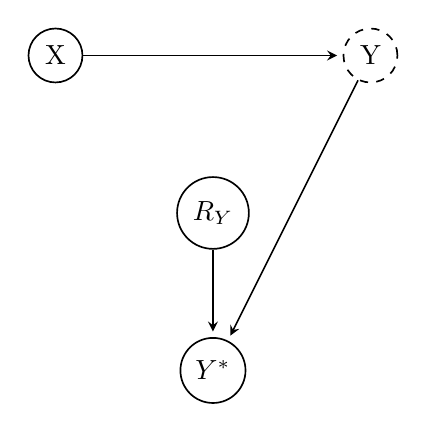
\begin{tikzpicture}[
            > = stealth, % arrow head style
            shorten > = 2pt, % don't touch arrow head to node
            auto,
            node distance = 3cm, % distance between nodes
            semithick % line style
        ]

\node[shape=circle,draw=black] (X) at (0,0) {X};
\node[shape=circle,draw=black, style=dashed] (Y) at (4,0) {Y};
\node[shape=circle,draw=black] (Y^*) at (2,-4) {$Y^*$};
\node[shape=circle,draw=black] (R_Y) at (2,-2) {$R_Y$};
 

 \path [->] (X) edge node[left] {} (Y);
 \path [->] (R_Y) edge node[left] {} (Y^*);
 \path [->] (Y) edge node[left] {} (Y^*);        
\end{tikzpicture}
\caption{"Hard" MNAR Case} \label{fig:MissingExternal}
\end{figure}
\end{example}

Given that recovery under missingness is sometimes possible with external data, we want to establish conditions which describe all cases in which recovery must be possible. We will describe such conditions for recovering both joint distributions and conditionals with or without external data.

 
\begin{theorem}
A conditional distribution $P(y | x)$ with $X, Y \in V_o \cup V_m$ is recoverable if and only if at least one on of the following statements holds:

\begin{enumerate}
\item $Y \in Vo$ and 
\end{enumerate}
\end{theorem}


%If you feel it necessary to include an appendix, it goes here.


%This is where endnotes are supposed to go, if you have them.
%I have no idea how endnotes work with LaTeX.

  \backmatter % backmatter makes the index and bibliography appear properly in the t.o.c...

% if you're using bibtex, the next line forces every entry in the bibtex file to be included
% in your bibliography, regardless of whether or not you've cited it in the thesis.
    \nocite{*}

% Rename my bibliography to be called "Works Cited" and not "References" or ``Bibliography''
% \renewcommand{\bibname}{Works Cited}

%    \bibliographystyle{bsts/mla-good} % there are a variety of styles available; 
%  \bibliographystyle{plainnat}
% replace ``plainnat'' with the style of choice. You can refer to files in the bsts or APA 
% subfolder, e.g. 
 \bibliographystyle{APA/apa-good}  % or
 \bibliography{thesis}
\nocite{*}% there are a variety of styles available; 
%  \bibliographystyle{plainnat}
% replace ``plainnat'' with the style of choice. You can refer to files in the bsts or APA 
% subfolder, e.g. 
%\bibliographystyle{APA/apa-good}  % or
 % Comment the above two lines and uncomment the next line to use biblatex-chicago.
 %\printbibliography[heading=bibintoc]
\appendix
\chapter{Appendix}

\section{Heckman}

\section{Deriving the Bias}

Heckman is viewing selection bias as being the result of an omitted variable which we can obtain. Here we give the derivation of what this variable actually is, closely following the original paper but with some clarifications and changes to notation as in \citep{Jin}. We know that:

$$E[Y | \mathbf{X}, S = 1] = E[ \mathbf{X} \boldsymbol{\beta} + \epsilon | \mathbf{X}, R_Y = 0] = \mathbf{X} \boldsymbol{\beta} + E[\epsilon |  \mathbf{X}, R_Y = 0].$$

Our independence assumption gives that $ E[\epsilon |  \mathbf{X}, S = 1] =  E[\epsilon |  R_Y = 0]$ and so this is the quantity we wish to estimate. Now, $S=1 \implies  \mathbf{W} \boldsymbol{\delta} + \tau > 0$ and we write:  

$$E[\epsilon |  \mathbf{X}, R_Y = 0 ] = E[\epsilon | \mathbf{W} \boldsymbol{\delta}+ \tau > 0] = E[\epsilon |  \tau > - \mathbf{W} \boldsymbol{\delta}].$$

Since $(\epsilon, \tau)$ follows a bivariate normal distribution and each have a marginal mean of $0$, the conditional expectation $E[\epsilon | \tau] = \rho \frac{\sigma_{\epsilon}}{\sigma_{\tau}} \tau$ where $\rho$ is the correlation between $\epsilon$ and $\tau$ and $\sigma^2_{\epsilon}$, $\sigma^2_{\tau}$ are the respective variances. Let $\gamma  = \rho \frac{\sigma_{\epsilon}}{\sigma_{\tau}}$ giving $E[\epsilon | \tau] = \gamma \tau$. Notice that when $\rho = 0$ (meaning $\epsilon$ and $\tau$ are independent), the $\gamma$ term is equal to $0$ and therefore the selection does not bias the estimate.  We may then apply the law of total expectation (sometimes call Adam's law):

$$E[\epsilon | \tau] = E[E[\epsilon | \tau] | \tau] = E[\gamma \tau | \tau] = \gamma E[\tau | \tau]$$	

So, when $\tau > - \mathbf{W} \boldsymbol{\delta}$, $E[\tau | \tau] = E[\tau | \tau > - \mathbf{W} \boldsymbol{\delta}]$ and we have that:

$$E[\epsilon | \tau >  - \mathbf{W} \boldsymbol{\delta}]  = \gamma E[ \tau | \tau >   - \mathbf{W} \boldsymbol{\delta}]$$																																																												
We recognize this as the expectation of a truncated normal, which is given by the inverse Mills ratio $E[X | X > x] = \sigma \frac{\phi(\frac{x- \mu}{\sigma})}{1 - \Phi(\frac{x - \mu}{\sigma})}$ for $X \sim N(\mu, \sigma^2)$. As usual, $\phi$ is the density function for the standard normal and $\Phi$ is the distribution function. By assumption, $\mu = 0$. Therefore,						

$$E[\epsilon | \tau > -\mathbf{W} \boldsymbol{\delta}] = \gamma \sigma_{\tau}\frac{\phi(\frac{-\mathbf{W} \boldsymbol{\delta}}{\sigma_\tau})}{1 - \Phi(\frac{-\mathbf{W} \boldsymbol{\delta}}{\sigma_\tau})}.$$				

So the bias term  we want to estimate is $\gamma\sigma_{\tau}\frac{\phi(\frac{-\mathbf{W} \boldsymbol{\delta}}{\sigma_\tau})}{1 - \Phi(\frac{-\mathbf{W} \boldsymbol{\delta}}{\sigma_\tau})}$. This is done in several parts \cite{Heckman_1979}.

Something to note: unlike the approach we see in the more contemporary selection bias literature, Heckman's method asks for external information on the selection mechanism itself, not the variables being measured. In addition to this, Heckman makes very strong parametric assumptions. Sometimes when such assumptions are made, the method is still relatively robust to (mild) violations.  However, Heckman's correction's does not generally have this property, and violations of the set-up can cause seriously biased estimates \citep{Little_1986}. This lack of robustness has led to Heckman's method becoming less popular in recent years \citep{Bushway_2007}.



\subsection{Examples}

Heckman developed his technique in the context of economic research, and its implementation typically relies on further assumptions justified by economic theory. Particularly, $Z$ is often understood as an \emph{unmeasured} continuous random variable following the linear regression assumptions \citep{Winship_Mare_1992}. Sometimes,  this variable is not directly measurable - such as an individual propensity or ability - that is nonetheless assumed to exist. We quickly review a number of  fairly standard  examples used to introduce Heckman's method \citep{Heckman_1979}, \citep{Guo_2015}.

\begin{enumerate}
\item Estimating the wages women not in the workforce would make if they entered the workforce using data for women currently in the workforce. Selection occurs because the women in the workforce differ from those who are not.

\item Estimating the effect of unionization of worker wages - similar to the last example, unionized workers might have joined the union because they were unsatisfied with their wages pre-unionization.

\item Estimating effects of schooling/training programs of worker productivity. Once again, the problem is that the people who choose to participate in such programs cannot be used to represent the workers who did not make that 
\end{enumerate}

In the spirit of some of these examples, we describe a relevant variation in more detail. Suppose that we are working with Reed College academic services to measure the effect of tutoring on student homework grades in the introductory chemistry sequence. We have collected a collected a set of relevant covariates ($\mathbf{X}$) on all students in the course such as major, high school grades, basic demographics, etc. The response variable ($\text{Grade Change}$) is the difference between the student's average homework scores before their first tutoring appointment and the average score after. Since some students do not seek tutoring, their value of $Y$ is missing. We assume that the response variable follows the linear regression assumptions:

$$\text{Grade Change} =   \mathbf{X}\boldsymbol{\beta} + \epsilon$$

For normally distributed $\epsilon$ with mean $0$. As students who participate in tutoring might differ from students who do not, it would be incorrect to use the model created using data for students that did seek tutoring to estimate the impact that tutoring would have on students who did not chose to be tutored. So, we must create a model for a student's probability of going to tutoring. To do this though Heckman's technique, we must further assume that a student seeks tutoring a when some unmeasured value crosses a threshold. There are multiple options here, and in practice this a stage that requires existing economic theory to be justified. In our case, these details are not important we assume that $\text{Tutoring Value}$ is, for each student, the perceived value of going to tutoring minus the students value of an equal amount of time for a different activity, such that a student goes to tutoring if  $\text{Tutoring Value}$ is positive. We have further collected from each student covariates capturing their motivation to do well in their courses, their perception of the usefulness of tutoring, and the amount of free time they have. Together with the covariates we measured for $X$, these variables constitute $\mathbf{\mathbf{W}}$,  and again we require linear regression assumptions are satisfied:

$$\text{Tutoring Desire} = \mathbf{W}  \boldsymbol{\delta} + \tau$$

With $\tau$ being normally distributed with mean $0$ such that $\epsilon$ and $\tau$ are jointly bivariate normal with correlation $\rho$. We can then implement the correction as follows:

\begin{enumerate}
\item Define the selection variable $S$ as $1$ for student with data for $\text{Grade Change}$ and $0$ for those who do not.

\item Create a probit model $P(S=1 | W)$ which yields as estimate of $\frac{\boldsymbol{\delta}}{\sigma_\tau}$ as the coefficients on $\mathbf{W}$.

\item We then estimate the inverse Mill's ratio $\frac{\phi(\frac{-\mathbf{W} \boldsymbol{\delta}}{\sigma_\tau})}{1 - \Phi(\frac{-\mathbf{W} \boldsymbol{\delta}}{\sigma_\tau})}$ and include the term in the regression equation, giving consistent estimates of $E[\text{Grade Change} | \mathbf{X}]$.
\end{enumerate}


 
\subsection{Conditional Expectation of Bivariate Normal Distribution}

We want to show that for $(\epsilon, \tau) \sim N((0,0), \boldsymbol{\Sigma})$ (where $\boldsymbol{\Sigma} = \begin{pmatrix}
\sigma_\epsilon^2 &\ \rho \sigma_\epsilon \sigma_\tau \\
\rho \sigma_\epsilon \sigma_\tau &\ \sigma_\tau^2
\end{pmatrix}$ and $\rho$ is the correlation of $\epsilon$ and $\tau$) the conditional $E[\epsilon | \tau] = \rho \frac{\sigma_\epsilon}{\sigma_\tau} \tau$. The normal distribution has the property that the covariance (therefore correlation) of determines the dependence structure. Consider the random variable $\epsilon - \frac{\rho}{\sigma_\tau} \tau$. We want to show that this random variable is independent of $\tau$. This is true when their covariance is $0$, i.e. when $E[\tau (\epsilon -\rho \frac{\sigma_\epsilon}{\sigma_\tau}\tau)] - E[\tau] E[\epsilon - \rho \frac{\sigma_\epsilon}{\sigma_\tau}  \tau] = 0$. In fact, since $E[\tau]=0$ by assumption, we want to show that $E[\tau (\epsilon -\rho \frac{\sigma_\epsilon}{\sigma_\tau} \tau)] = 0$

We have:

\begin{align*}
E[\tau (\epsilon - \rho \frac{\sigma_\epsilon}{\sigma_\tau} \tau)] &= E[\tau \epsilon] -  \rho \frac{\sigma_\epsilon}{\sigma_\tau} E[\tau^2] \\
&=  \rho \sigma_\tau \sigma_\epsilon -  \rho \frac{\sigma_\epsilon}{\sigma_\tau}E[\tau^2] \\ 
&= \rho \sigma_\tau \sigma_\epsilon -  \rho \sigma_\tau \\
&= 0
\end{align*}
As desired. Then, applying independence, we have that:

\begin{align*}
E[\epsilon | \tau] &= E[\epsilon - \frac{\rho}{\sigma_\tau} \tau +  \frac{\rho}{\sigma_\tau} \tau | \tau] \\
&= E[\epsilon - \rho \frac{\sigma_\epsilon}{\sigma_\tau} \tau | \tau] + E[\rho \frac{\sigma_\epsilon}{\sigma_\tau} \tau | \tau] \\
&= E[\epsilon - \rho \frac{\sigma_\epsilon}{\sigma_\tau} \tau] +\rho \frac{\sigma_\epsilon}{\sigma_\tau}E[\tau | \tau] \\
&= E[\epsilon] + \rho \frac{\sigma_\epsilon}{\sigma_\tau} \tau \\
&= \rho \frac{\sigma_\epsilon}{\sigma_\tau} \tau. 
\end{align*}

\subsection{Truncated Normal and the Inverse Mills Ratio}

We show that $E[\tau | \tau \geq t] = \sigma_\tau \frac{\phi(t)}{1 - \Phi(t)}$. By the definition of truncated density, the truncated PDF $f_{\tau | \tau > t}$ is:

$$f_{\tau | \tau > t}(x) = \frac{f_\tau(x)}{1 - F_\tau(t)} \text{  for } x > t$$

Where $f$ is the density function for $\tau$ and $F$ is the distribution function for $\tau$. In particular, these are $f(x) = \frac{1}{\sigma_\tau} \phi(\frac{x}{\sigma_\tau})$ and $F(x) = \Phi(\frac{x}{\sigma_\tau})$ giving $f_{\tau | \tau > t}(x) = \frac{\phi(\frac{x}{\sigma_\tau})}{\sigma_\tau(1 - \Phi(\frac{t}{\sigma_\tau}))} \text{  for } x > t$. To find the expected value, we integrate. 

\begin{align*}
E[\tau | \tau > - t] &= \int_t^\infty x f_{\tau | \tau > t}(x) \\
&= \int_t^\infty \frac{\phi(\frac{x}{\sigma_\tau})}{\sigma_\tau(1 - \Phi(\frac{t}{\sigma_\tau}))} \\
&= \frac{1}{\sigma_\tau(1 - \Phi(\frac{t}{\sigma_\tau}))} \int_t^\infty x \phi(\frac{x}{\sigma_\tau})  \\
&= \frac{1}{\sigma_\tau(1 - \Phi(\frac{t}{\sigma_\tau}))} \int_t^\infty  \frac{x}{\sigma_\tau \sqrt{2 \pi}}e^{-\frac{x^2}{2 \sigma_\tau^2}} \\
&= \frac{1}{\sigma_\tau(1 - \Phi(\frac{t}{\sigma_\tau}))} \left( -\dfrac{{\sigma_\tau}e^{-\frac{x^2}{2{\sigma_\tau}^2}}}{\sqrt{{2\pi}}} \bigg |_t^\infty \right) \\
&= \frac{1}{\sigma_\tau(1 - \Phi(\frac{t}{\sigma_\tau}))} \dfrac{{\sigma_\tau}e^{-\frac{t^2}{2{\sigma_\tau}^2}}}{\sqrt{{2\pi}}}  \\
&= \frac{\sigma_\tau^2 \phi(\frac{t}{\sigma_\tau})}{\sigma_\tau(1 - \Phi(\frac{t}{\sigma_\tau}))} \\
&= \sigma_\tau  \frac{\phi(\frac{t}{\sigma_\tau})}{(1 - \Phi(\frac{t}{\sigma_\tau}))} 
\end{align*}
Which is the desired result.


% Finally, an index would go here... but it is also optional.
\end{document}
